\documentclass[mat1, tisk]{fmfdelo}
% \documentclass[fin1, tisk]{fmfdelo}
% Če pobrišete možnost tisk, bodo povezave obarvane,
% na začetku pa ne bo praznih strani po naslovu, …

%%%%%%%%%%%%%%%%%%%%%%%%%%%%%%%%%%%%%%%%%%%%%%%%%%%%%%%%%%%%%%%%%%%%%%%%%%%%%%%
% METAPODATKI
%%%%%%%%%%%%%%%%%%%%%%%%%%%%%%%%%%%%%%%%%%%%%%%%%%%%%%%%%%%%%%%%%%%%%%%%%%%%%%%

% - vaše ime
\avtor{Jaša Knap}

% - naslov dela v slovenščini
\naslov{Kratki zakoni v grupah}

% - naslov dela v angleščini
\title{Short Group Laws}

% - ime mentorja/mentorice s polnim nazivom:
%   - doc.~dr.~Ime Priimek
%   - izr.~prof.~dr.~Ime Priimek
%   - prof.~dr.~Ime Priimek
%   za druge variante uporabite ustrezne ukaze
\mentor{doc.~dr.~Urban Jezernik}
% \somentor{...}
% \mentorica{...}
% \somentorica{...}
% \mentorja{...}{...}
% \somentorja{...}{...}
% \mentorici{...}{...}
% \somentorici{...}{...}

% - leto diplome
\letnica{2024} 

% - povzetek v slovenščini
%   V povzetku na kratko opišite vsebinske rezultate dela. Sem ne sodi razlaga
%   organizacije dela, torej v katerem razdelku je kaj, pač pa le opis vsebine.

% Dvočrkovni zakon v grupi $G$ je abstrakten produkt elementov $x$, $y$ ter njunih inverzov $x^{-1}$ in $y^{-1}$, ki ima lastnost, da za vsako zamenjavo $x$ in $y$ s konkretnima
% elementoma $g, h \in G$ dobimo rezultat $1 \in G$. Na primer beseda $xyx^{-1}y^{-1}$ je zakon v grupi natanko tedaj, ko je grupa Abelova. Tema diplomske naloge je ocenjevanje asimtotske rasti dolžine najkrajših netrivialnih zakonov za specifične družine grup, še posebej družine $\operatorname{PSL}_2(q)$ in družine nilpotentnih grup določenega razreda nilpotentnosti. Proti koncu se naloga dotakne tudi računalniškega iskanja zakonov. 

\povzetek{TODO}

% - povzetek v angleščini
\abstract{TODO}

% - klasifikacijske oznake, ločene z vejicami
%   Oznake, ki opisujejo področje dela, so dostopne na strani https://www.ams.org/msc/
\klasifikacija{20, 05C81} % TODO

% - ključne besede, ki nastopajo v delu, ločene s \sep
\kljucnebesede{...\sep ...} % TODO

% - angleški prevod ključnih besed
\keywords{...\sep ...} % angleški prevod ključnih besed % TODO

% - angleško-slovenski slovar strokovnih izrazov
% TODO
\slovar{
% \geslo{angleški izraz}{slovenski izraz}
% ...
}

% - ime datoteke z viri (vključno s končnico .bib), če uporabljate BibTeX
\literatura{literatura.bib}

%%%%%%%%%%%%%%%%%%%%%%%%%%%%%%%%%%%%%%%%%%%%%%%%%%%%%%%%%%%%%%%%%%%%%%%%%%%%%%%
% DODATNE DEFINICIJE
%%%%%%%%%%%%%%%%%%%%%%%%%%%%%%%%%%%%%%%%%%%%%%%%%%%%%%%%%%%%%%%%%%%%%%%%%%%%%%%

% naložite dodatne pakete, ki jih potrebujete
% \usepackage{...}

\usepackage{tikz}
\usepackage{cancel}

% deklarirajte vse matematične operatorje, da jih bo LaTeX pravilno stavil
% \DeclareMathOperator{\...}{...}

\newcommand{\bigslant}[2]{{\raisebox{.2em}{$#1$}\left/\raisebox{-.2em}{$#2$}\right.}}

\numberwithin{equation}{section}  % števec za enačbe zgleda kot (2.7) in se resetira v vsakem razdelku
\newenvironment{skica}[1][Skica dokaza]{\begin{proof}[#1]}{\end{proof}}

% vstavite svoje definicije ...
% \newcommand{\...}{...}

%%%%%%%%%%%%%%%%%%%%%%%%%%%%%%%%%%%%%%%%%%%%%%%%%%%%%%%%%%%%%%%%%%%%%%%%%%%%%%%
% ZAČETEK VSEBINE
%%%%%%%%%%%%%%%%%%%%%%%%%%%%%%%%%%%%%%%%%%%%%%%%%%%%%%%%%%%%%%%%%%%%%%%%%%%%%%%

\begin{document}

\section{Uvod}

% TODO Vse izraze, ki jih uvedemo v definicijah, trditvah ali v veznem besedilu, pišemo poudarjeno, torej znotraj ukaza \emph{...}


% TODO tale uvod je treba še kar lepo urediti, da bo v smiselni obliki
% treba je popraviti definicijo zakona, trenutno ni najbolj logično ...
% treba je obrazložiti kaj je sploh poanta diplome

Dvočrkovni zakon v grupi $G$ je abstrakten produkt elementov $x$, $y$ ter njunih inverzov $x^{-1}$ in $y^{-1}$, ki ima lastnost, da za vsako zamenjavo $x$ in $y$ s konkretnima
elementoma $g, h \in G$ dobimo rezultat $1 \in G$.

\begin{opomba}
Definicijo $n$-črkovnih zakonov dobimo tako, da v zgornji definiciji elementa $x$, $y$ (in njuna inverza) nadomestimo z elementi $x_1, x_2, \ldots, x_n$ (in njihovimi inverzi),
ki jih zamenjujemo s konkretnimi elementi $g_1, g_2, \ldots, g_{n} \in G$.
\end{opomba}

\noindent
Zakonu $1$ pravimo trivialni zakon, ki v kontekstu raziskovanja zakonov ni posebej zanimiv. Najosnovnejši primer netrivialnega zakona se pojavi pri Abelovih grupah, kjer za poljubna elementa $x,y \in  G$ velja $xy = yx$, kar je ekvivalentno
zahtevi \begin{equation*}
xyx^{-1}y^{-1} = [x,y] = 1.
\end{equation*}

\noindent
Grupa $G$ je torej Abelova natanko tedaj, ko je štiričrkovna beseda $xyx^{-1}y^{-1}$ v njej zakon. 


\section{Osnovni pojmi}

Definicijo zakona \ref{def_zakon_osnovna} lahko bolj formalno zapišemo s pomočjo prostih grup.

\begin{definicija}
\label{def_prosta_grupa}
Naj bo $S$ množica. Grupa $F(S)$ je (do izomorfizma natančno) enolična grupa z lastnostjo, da za poljubno grupo $G$ in poljubno preslikavo
$\varphi: S \to G$ obstaja natanko ena razširitev $\varphi: F(S) \to G$, ki je hkrati homomorfizem grup. 
\end{definicija}

\begin{opomba}
Za poljubni množici $S$ in $T$ velja $F(S) \cong F(T)$ natanko tedaj, ko $\lvert S \rvert = \lvert T \rvert$. Zato lahko v primeru končne množice $\lvert S \rvert = k$ govorimo o 
prosti grupi ranga $k$, ki jo označimo z $F_k$.
\end{opomba}

\noindent
V viru (\cite[str.~4, tridtev 1.9]{Lyndon_Schupp_2015}) je natančno razloženo znano dejstvo, da lahko elemente proste grupe $F(S)$ predstavimo v obliki okrajšanih besed,
torej besed oblike $w = s_1 \cdots s_n$, kjer je $s_i \in S \cup S^{-1}$ za $i = 1, \ldots, n$ in $s_i \neq s_{i+1}^{-1}$ za $i = 1, \ldots, n-1$. Tu je $S^{-1} = \left\{ s^{-1}  \middle|\, s \in  S \right\}$.
Z upoštevanjem tega dejstva lahko elementom proste grupe $F(S)$ določimo dolžino.

\begin{definicija}
\label{def_dolzina_besede}
Naj bo $w \in  F(S)$ element proste grupe nad množico $S$ in naj bo njegova okrajšana oblika $w = s_1 \cdots s_n$. Potem številu $n$ pravimo dolžina (besede) $w$ in pišemo $l(w) = n$.
\end{definicija}

\noindent
Zdaj definiramo izginjajočo množico besede $w$ v grupi $G$.

\begin{definicija}
\label{def_izginjajoca_mnozica}
Naj bo $w \in  F_k$. Potem množico \begin{equation*}
Z(G, w) := \left\{ (g_1, .., g_{k}) \in  G^{k}  \middle|\, w(g_1, \ldots, g_{k}) = 1 \right\} 
\end{equation*}  
imenujemo izginajoča množica besede $w$ v grupi $G$. Tu $1$ označuje enoto v grupi $G$, $w(g_1, \ldots, g_{k})$ pa sliko elementa $w \in F_k = \langle a_{1}, \ldots , a_k \rangle$ s homomorfizmom,
induciranim s preslikavo $\varphi: a_{i} \mapsto g_{i}$ za $i = 1,\ldots, n$ v skladu z definicijo \ref{def_prosta_grupa}.  
\end{definicija}

\indent
Zdaj lahko natančno formuliramo definicjo zakona. .

\begin{definicija}\label{def_zakon_formalna}
Beseda $w \in F_k$ je $k$-črkovni zakon v grupi $G$, če je $Z(G, w) = G^{k}$. Alternativno, beseda $w \in F_k$ je $k$-črkovni zakon v grupi $G$, če jo vsak homomorfizem $\varphi: F_k \to G$ slika v enoto $1 \in G$.   
\end{definicija}

Definirajmo še zakon v podmnožici grupe.
\begin{definicija}
    \label{def_zakon_v_podmnožici}
    Naj bo $G$ grupa in $H$ njena podmnožica. Beseda $w \in F_k$ je zakon v podmnožici $H$, če za vse izbire $g_1, \ldots, g_k \in H$ velja $w(g_1, \ldots, g_{k}) = 1_G$.
    \end{definicija}
    
    \begin{opomba}
    Beseda $w \in F_k$ je zakon v podmnožici $H \subseteq G$ natanko tedaj, ko je $Z(G, w) \supseteq H^{k}$ ter zakon v vsaki podmnožici $H_1, \ldots, H_n \subseteq G$ natanko tedaj, ko je $Z(G, w) \supseteq \bigcup_{i = 1}^{n} H_i^{k}$.  
    \end{opomba}

Ta definicija nam omogoča vpogled v strukturo zakonov. Naj $K(k) \subseteq F_k$ označuje množico $k$-črkovnih zakonov. Potem v luči prejšnje definicije velja
\begin{equation*}
K(k)  = \bigcap_{\varphi: F_k \to G} \ker(\varphi).   
\end{equation*}  
Ta množica je končni presek edink v $G$ in posledično tudi sama edinka. Še več, invariantna je za vsak avtomorfizem $\alpha: F_k \to  F_k$, saj
\begin{equation*}
    K(k)  = \bigcap_{\varphi: F_k \to G} \ker(\varphi) = \bigcap_{\varphi: F_k \to G} \ker(\varphi \circ \alpha). 
\end{equation*}  
To je preprosta posledica dejstva, da $\varphi$ preteče grupo $\operatorname{Hom}(F_k, G)$ natanko tedaj, ko jo preteče $\varphi \circ \alpha$.     

\begin{lema}\label{lem_koncni_indeks_koncnega_preseka}
Naj bo $G$ grupa ter $H_1, \ldots, H_n$ njene podgrupe končnega indeksa, torej $[G: H_i] < \infty$ za $i = 1, \ldots, n$. Potem je tudi $\bigcap_{i = 1}^{n} H_i$ podgrupa končnega indeksa v $G$ in velja
\begin{equation*}
\left[ G: \bigcap_{i = 1}^{n} H_i \right]  \le \prod_{i=1}^{n} [G: H_i].  
\end{equation*} 
\end{lema}

\begin{dokaz}
Dovolj je dokazati trditev za $n = 2$, za višje vrednosti sledi z indukcijo. Naj bosta $H_1, H_2 \le G$ podgrupi končnega indeksa, označimo $S: = H_1 \cup H_2$. Naj bosta $C_1$ in $C_2$ množici odsekov podgrup $H_1$ in $H_2$ v $G$ ter naj bo $C$ množica odsekov podgrupe $S$ v $G$. Definiramo preslikavo $f : C \to  C_1 \times C_2$ s predpisom $f(g S ) = (g H_1, g H_2)$. Desna smer sklepa \begin{equation*}
 g S = h S \iff gh^{-1} \in H_1, \, gh^{-1} \in H_2  \iff g H_1 = h H_1, \, g H_2 = h H_2
\end{equation*}  
nam podaja dobro definiranost, leva pa injektivnost preslikave $f$, ki nam da $\lvert C \rvert \le  \lvert C_1 \rvert \lvert C_2 \rvert $.    
\end{dokaz}
Z uporabo te leme direktno sledi, da je grupa $K(k)$ podgrupa končnega indeksa v $F_k$. To dejstvo bo še posebej pobmembno pri iskanju zakonov z računalnikom.

\begin{definicija}\label{def_ozina}
Število \begin{equation*}
\operatorname{girth}_{k}(G) := \min \left\{ l(w)  \middle|\,  w \in F_k \setminus \left\{ 1\right\} \text{ je zakon v } G  \right\} \cup \left\{ \infty\right\} 
\end{equation*}  
je $k$-črkovna dolžina grupe $G$.  
\end{definicija}

% TODO tukaj poveži ožino grafa z bistvom naloge, morda poveži z https://www.researchgate.net/publication/2441748_On_The_Girth_Of_Groups

\begin{definicija}
\label{def_cayleyev_graf}
Naj bo $G$ grupa in $S \subseteq G$ njena podmnožica, za katero velja $S = S^{-1}$. Potem $\operatorname{Cay}(G, S)$ označuje graf z vozlišči $V = G$ in povezavami
$E = \left\{ (p, q) \middle|\, p^{-1}q \in  S \right\}$. Imenujemo ga Cayleyjev graf grupe $G$, generiran z množico $S$.  
\end{definicija}

\begin{opomba}
Pogoj simetričnosti $S = S^{-1}$ nam pove, da je $\operatorname{Cay}(G, S)$ pravi graf in ne zgolj usmerjen. Imamo namreč \begin{equation*}
(p,q) \in  E \iff p^{-1}q \iff q^{-1}p \iff (q,p) \in  E.
\end{equation*}  
\end{opomba}

\begin{primer}
Na spodnjih slikah imamo Cayleyjev graf grupe diedrske grupe $D_{10} = \langle r, Z \rangle$ za različni generatorski množici.
TODO nariši desno od tega še graf s 5 generatorji, morda raje Cayleyjev graf proste grupe F2, saj nastopa naslednji trditvi
\begin{center}
    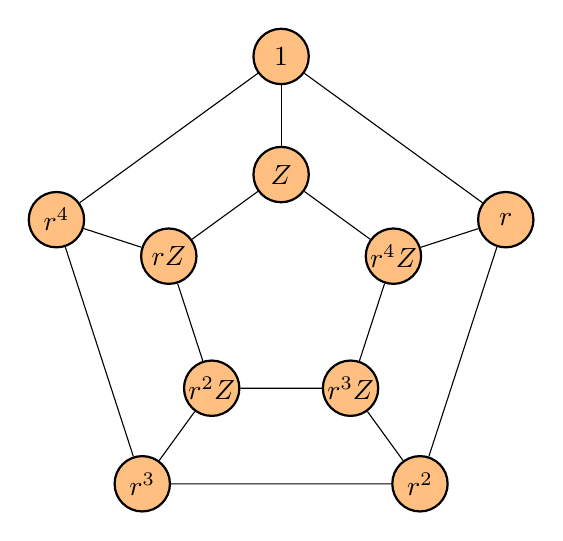
\begin{tikzpicture}[rotate=90, scale=1.5]
    \tikzset{vertex/.style={draw, thick, circle, fill=orange!50, minimum size=20pt, inner sep=0pt}}
    
    \node[vertex] (v1) at (-0*360/5:1) {$Z$};
    \node[vertex] (v2) at (-0*360/5:2) {$1$};
    \node[vertex] (v3) at (-1*360/5:1) {$r^4Z$};
    \node[vertex] (v4) at (-1*360/5:2) {$r$};
    \node[vertex] (v5) at (-2*360/5:1) {$r^3Z$};
    \node[vertex] (v6) at (-2*360/5:2) {$r^2$};
    \node[vertex] (v7) at (-3*360/5:1) {$r^2Z$};
    \node[vertex] (v8) at (-3*360/5:2) {$r^3$};
    \node[vertex] (v9) at (-4*360/5:1) {$rZ$};
    \node[vertex] (v10) at (-4*360/5:2) {$r^4$};
    
    \draw (v1) -- (v2);
    \draw (v1) -- (v3);
    \draw (v2) -- (v4);
    \draw (v3) -- (v4);
    \draw (v3) -- (v5);
    \draw (v4) -- (v6);
    \draw (v5) -- (v6);
    \draw (v5) -- (v7);
    \draw (v6) -- (v8);
    \draw (v7) -- (v8);
    \draw (v1) -- (v9);
    \draw (v7) -- (v9);
    \draw (v2) -- (v10);
    \draw (v8) -- (v10);
    \draw (v9) -- (v10);
    \end{tikzpicture}
    \end{center}
\end{primer}


\begin{opomba}
Ime ožina je smiselno v kontekstu definicije Cayleyjevega grafa grupe. TODO zakaj
\end{opomba}


Izkaže se, da so najbolj zanimivi in za obravnavo relevantni dvočrkovni zakoni. To nam sporočata naslednji dve trditvi.
\begin{trditev}
\label{trd_vlozitev_proste_grupe}
 Obstaja vložitev grupe $F_{2 \cdot 3^{k}} = \langle x_1, \ldots, x_{2 \cdot 3^{k}} \rangle$ v grupo $F_2 = \langle x,y \rangle $, da velja $l(x_i) = 2k + 1$, kjer $l(w)$ označuje dolžino besede $w \in F_2 = \langle x,y \rangle$. 
\end{trditev}


\begin{dokaz}
    Dokaz trditve je nekoliko preveč tehničen za potrebe te naloge, naveden v~\cite{Schneider_2016}. Glavna ideja je, da obravnavamo Cayleyev graf proste grupe $F_2$ z dvema generatorjema.
Drevo vseh besed dolžine $k$ na ustrezen način dopolnimo tako, da dodamo povezave listom. Pri tem dobimo cikle dolžine $2k + 1$ in utemeljimo, da lahko jih lahko obravnavamo kot elemente $F_{2 \cdot 3^{k}}$, vložene v $F_2$. 
\end{dokaz}


\begin{posledica}\label{psl_veccrkovni_zakoni_meje}
Naj bo $G$ grupa in $k \ge 2$ naravno število. Potem velja \begin{equation*}
     \operatorname{girth}_{k}(G) \le  \operatorname{girth}{2}(G) 
\end{equation*}  
in \begin{equation*}
\operatorname{girth}_{2}(G) \le \left( {2 \left\lceil \log_3(\frac{k}{2}) \right\rceil + 1  } \right) \operatorname{girth}_{k}(G).
\end{equation*}  
\end{posledica}
\begin{dokaz}
    Prva neenakost je očitna, saj so vsi dvočrkovni zakoni tudi $k$-črkovni zakoni. Druga neenakost drži, saj lahko po prejšnji trditvi vložimo $F_{{2 \left\lceil \log_3(\frac{k}{2}) \right\rceil}}$ v $F_2$
    tako, da noben generator ni daljši od ${2 \left\lceil \log_3(\frac{k}{2}) \right\rceil + 1  }$. Hkrati velja $F_k \subseteq F_{{2 \left\lceil \log_3(\frac{k}{2}) \right\rceil}}$, kar nam da želeno neenakost.
\end{dokaz}


\section{Teorija naključnih sprehodov}

Za obravnavo zakonov v simetričnih grupah bomo potrebovali naključne sprehode, natančneje lene naključne sprehode (TODO poglej, če se res tako imenuje).
Naj bo grupa $G$ generirana s simetrično podmnožico $S \subseteq G$. Tekom tega razdelka naj bo $\Gamma = \operatorname{Cay}(G, S)$, ki je po prejšnjem premisleku (TODO dokaz, da je Cayleyjev graf regularen in povezan).

\begin{definicija}
\label{def_leni_nakljucni_sprehod}
    Leni naključni sprehod je naključno zaporedje elementov $w_n \in S$ za $n \in \mathbb{N} \cup \left\{ 0\right\} $, porojeno s formulo \begin{equation*}
        \mathbb{P}(w_{n+1} = g   \vert \,  w_n = h) = \begin{cases}
            \frac{1}{2}; & \text{če }  g = h, \\
            \frac{1}{2 \lvert S \rvert }; & \text{če } g = sh \text{ za neki } s \in S.
        \end{cases}
    \end{equation*}  
\end{definicija}
Na vsakem koraku lenega naključnega sprehoda se torej z verjetnostjo $1 / 2$ element ne spremeni, z verjetnostjo $1 / 2$ pa se naključno spremeni v enega od svojih sosedov, ki jih je $\lvert S \rvert$.
To lahko opišemo tudi z matrikami. Recimo, da je $u_n$ vejretnostna porazdelitev $\lvert G \rvert$ razsežnega vektorja, ki predstavlja vozlišča grafa $\Gamma$, po $n$-tem koraku in recimo, da začetno porazdelitev $u_0$ poznamo. Dalje, definiramo matriko lenega naključnega sprehoda $M \in M_{\lvert G \rvert }(\mathbb{R})$, s predpisom    
\begin{equation*}
M = \frac{1}{2} \left(I + \frac{1}{\lvert S \rvert } A \right) = \frac{1}{2} (I + \tilde{A}),
\end{equation*}  
kjer smo z $A$ označili matriko soseščine grafa $\Gamma$, z $\tilde{A}$ pa smo označili matriko $\frac{1}{\lvert S \rvert} A$, da . Ni težko premisliti, da po definiciji \ref{def_leni_nakljucni_sprehod} sledi zveza 
\begin{equation*}
u_n = M^{n} u_0,
\end{equation*}  
ki nam omogoča vpogled v lastnosti naključnih sprehodov. 

\begin{lema}
\label{lem_M_je_sebiadjungirana}
Matrika $M$ je diagonalizabilna, sebiadjungirana in njene lastne vrednosti ležijo v intervalu $[0, 1]$.
\end{lema}
\begin{dokaz}
Ker je realna matrika $M$ simetrična, je diagonalizabilna, sebiadjungirana in velja, da so vektorji, ki pripadajo paroma različnim lastnim vrednostim, med seboj ortogonalni. Enako velja za matriko $A$. Sebiadjungiranost nam implicira realnost lastnih vrednosti matrik $M$ in $A$.
Z oceno matričnih norm \begin{equation*}
    \sqrt{ \lambda_{\max} (\tilde{A}^2)} = \sqrt{\lambda_{\max} (\tilde{A}^{T} \tilde{A} )}  = \lvert\lvert \tilde{A} \rvert\rvert_2 \le \sqrt{\lvert\lvert A \rvert\rvert_1}  \lvert\lvert \tilde{A} \rvert\rvert_{\infty} = 1 
\end{equation*}  
sledi, da ima matrika $\tilde{A}$ lastne vrednosti v intervalu $[-1 ,1]$, kar pomeni, da lastne vrednosti matrike $M$ ležijo v intevalu $[0, 1]$. 
\end{dokaz}

Ker vemo, da so vse lastne vrednosti realne, jih lahko po razvrstimo po velikosti: 
\begin{equation*}
1 \ge \lambda_1(G, S) \ge \lambda_2(G, S) \ge \ldots \ge \lambda_{\lvert G \rvert }(G, S).  
\end{equation*}  
Izkaže se, da je glede na izbiro grupe $G$ in njene generirajoče množice $S$ lastna vrednost $\lambda_1(G, S) = 1 > \lambda_2(G, S)$. (TODO, posledica tega, da je $\Gamma$ povezan + konvergence zaporedja)
Razliko $1 - \lambda_2(G, 2)$ imenujemo \emph{spektralna razlika} grafa $\Gamma$. 

\begin{definicija}
\label{def_diameter_cayleyjevega_grafa}
Diameter Cayleyjevega grafa $\Gamma = \operatorname{Cay}(G, S)$ je število \begin{equation*}
    \operatorname{diam}(G, S) := \min \left\{ n \in \mathbb{N}  \middle|\, \forall g \in G. \exists s_1, \ldots , s_n \in S \cup \left\{ 1_G \right\} . g = s_1 \cdots s_n \right\} 
\end{equation*}  
\end{definicija}
Intuitivno nam diameter Cayleyjevega grafa poda najmanjše število korakov, po katerem lahko naključni sprehod po grafu $\Gamma$ doseže poljubni element grupe $G$. Za vse končnogenerirane in posledično končne grupe je diameter dobro definiran.
Za ocenjevanje dolžin zakonov v grafih je bistvena sledeča zveza med diametrom grafa in spektralno razliko lenega naključnega sprehoda.

\begin{trditev}
\label{trd_zveza_med_diametrom_grafa_in_spektralno_razliko}
 Velja zveza \begin{equation*}
 1 - \lambda_1(G, S) \ge \frac{1}{2 \lvert S \rvert \operatorname{diam}(G, S)^2}.
 \end{equation*}  
\end{trditev}
\begin{dokaz}
% TODO najdi referenco za dokaz te leme, oz si poglej vir, na katerega se sliče Thom
\end{dokaz}

Od tod sledi pomembna posledica \begin{posledica}
\label{psl_posledica_zveze_diameter}
Naj bo vektor $u = \frac{1}{\lvert G \rvert} I$ in naj bo $e_1$ bazni vektor enote $1_G$ (TODO tole bolje razloži). Potem velja ocena \begin{equation*}
\lvert M^{n} e_1 - u \rvert \le \lambda_1(G, S) \le \left( 1 - \frac{1}{2 \lvert S \rvert \operatorname{diam}(G, S)^2 } \right)^{n}. 
\end{equation*}    
\end{posledica}
\begin{dokaz}
Desna neenakost je direktna posledica trditve \ref{trd_zveza_med_diametrom_grafa_in_spektralno_razliko}. (TODO zakaj leva stran enačbe ... to bi se moralo dati intuitivno dokazati )
\end{dokaz}

Za konec potrebujemo še zadnjo lemo. \begin{equation*}
Naj bo $E$ podmnožica grupe $G$ in naj bo $\alpha := \lvert E \rvert / \lvert G \rvert$ in naj bo $(w_n)_{n \in  \mathbb{N}}$ leni naključni sprehod.
Če velja ocena \begin{equation*}
n \ge 2 \lvert S \rvert \operatorname{diam}(G, S)^2 \log(2 \lvert G \rvert ), 
\end{equation*}  
    velja $\mathbb{P}(w_n \in E) \ge \alpha / 2$.
\end{equation*}  
\begin{dokaz}
TODO, to je Cauchy--Schwarz
\end{dokaz}

% TOOD tukaj poveži besedilo z intuitivno razloago

Glavni rezultat, ki zagotovi obstoj kratkih zakonov, je Helfgott--Seressov izrek. \begin{equation*}
Naj par $(\sigma, \tau) \in S_n^2$ generira grupo $S_n$, torej $\langle \sigma, \tau \rangle = S_n$. Potem je diameter grafa $\Gamma = \operatorname{Cay}(S_n, \left\{ \sigma^{\pm 1}, \tau^{\pm 1} \right\} )$ največ \begin{equation*}
\exp(C \log(n)^{4} \log(\log(n))).
\end{equation*}  
Dokaz tega izreka je zelo težek in se moćno nanaša na klasifikacijo končnih enostavnih grup, zato ga opuščamo. Bralec ga lahko najde v \cite{Helfgott_Seress_2013}.
\section{Komutatorska in razširitvena lema}

\subsection{Komutatorska lema}



Recimo, da poznamo zakone v nekaterih podmnožicah grupe $G$, zanima pa nas, kako bi iz njih zgradili zakone za večje podmnožice te grupe. Na to vprašanje odgovarjata komutatorska in razširitvena lema,
ki sta ključni orodji pri obravnavanju zakonov.

\begin{definicija}\label{def_netrivialna_potenca}
Naj bo $G$ grupa. Element $g \in  G$ je netrivialna potenca, če obstajata $h \in G$ in naravno število $n > 1$, da je $g = h^{n}$.
\end{definicija}

% \begin{lema}[\cite{Lyndon_Schupp_2015}[str.~8, trditev 2.6]]\label{lem_uporaba_nielsen}
% Vsaka končnogenerirana podgrupa proste grupe je prosta.   
% \end{lema}
% % \begin{skica}
% %     -najprej Nielsenove transformacije
% %     -nato N-okrajšanost
% %     -ideja, da lahko prevedeš vse U na N-okrajšane
% %     -lema, da N-okrajšane ravno pravšnje
% % Ta lema je posebni primer Nielsen-Schreierjevega izreka, ki trdi, da je vsaka podgrupa proste grupe prosta \cite{Lyndon_Schupp_2015}[str.~8, trditev 2.11]. Njen dokaz je podan na straneh 5--7 v istega vira,  

% % \end{skica}

% \noindent
% Ta lema je posebni primer klasičnega Nielsen--Schreierjevega izreka, ki pravi, da je vsaka podgrupa proste grupe prosta. Dokazana je v \cite{Lyndon_Schupp_2015}[5--7] z uporabo Nielsenovih transformacij. 

% \begin{lema}
%     \label{lem_komutatorska_lema}
%      Naj bo $k \ge 2$, $e \in  \mathbb{N}$ in naj bodo besede $w_1, \ldots, w_m \in F_k$ netrivialne, pri čemer je $m = 2^{e}$. Potem obstaja beseda $w \in F_k$
%      dolžine \begin{equation*}
%      l(w) \le 2m \left(m + \sum_{i=1}^{m} l(w_{i}) \right),
%      \end{equation*}  
%     ki ni netrivialna potenca, da za vsako grupo $G$ velja \begin{equation*}
%     Z(G, w) \supseteq \operatorname{Z}(G, w_1) \cup \ldots \cup \operatorname{Z}(G, w_m).
%     \end{equation*}       
% \end{lema}
%     \begin{dokaz}
%         Dokaz poteka z indukcijo po $e \in  \mathbb{N}$. Naj bo $F_k = \langle S \rangle$.  Za $e = 0$ (oziroma $m = 1$) vzamemo $w = [s, w_1]$, kjer je $s \in S$ takšen element, da $w_1$ ni potenca $s$. To lahko storimo zaradi pogoja $k \ge 2$. Zaradi ustrezne izbire komutator $[s, w_1]$ ne more biti netrivialna potenca, njegova dolžina pa je kvečjem $2(l(w_1)  + 1)$.
%         Hkrati za poljubno grupo $G$ velja $\operatorname{Z}(G, w) \supseteq \operatorname{Z}(G, s) \cup \operatorname{Z}(G, w_1)$.
        
%         Zdaj se lotimo indukcijskega koraka v primeru $e \ge 1$ oziroma $m \ge 2$. Naj bodo podane besede $w_1, \ldots, w_{m / 2}, w_{m / 2 + 1}, \ldots, w_{2m}$. Po indukcijski predpostavki obstajata besedi $v_1, v_2 \in  F_{k}$, ki nista netrivialni potenci, da velja
%         \begin{equation*}
%         l(v_1) \le m \left(\frac{m}{2} + \sum_{i=1}^{m / 2} l(w_{i}) \right),
%         \end{equation*}  
%         \begin{equation*}
%             l(v_2) \le m \left(\frac{m}{2} + \sum_{i= m / 2 + 1}^{m} l(w_{i}) \right)
%         \end{equation*}  
%         in \begin{equation*}
%         \operatorname{Z}(G, v_1) \supseteq \operatorname{Z}(G, w_1) \cup \ldots \cup \operatorname{Z}(G, w_{m / 2}),
%         \end{equation*}  
%         \begin{equation*}
%             \operatorname{Z}(G, v_2) \supseteq \operatorname{Z}(G, w_{m / 2 + 1}) \cup \ldots \cup \operatorname{Z}(G, w_{m})
%         \end{equation*}  
%         za vsako grupo $G$.

%         Zdaj moramo le še utemeljiti, da lahko besedi $v_1$ ter $v_2$ ustrezno združimo. Vemo, da je komutator $[a,b]$ za $a,b \in F_k \setminus \left\{ 1\right\}$ trivialen natanko tedaj, ko $a$ in $b$ generirata prosto grupo ranga $1$. Po lemi \ref{lem_uporaba_nielsen} namreč vemo, da je podgrupa $\langle a, b \rangle \le F_k$ prosta,
%         hkrati pa $a$ in $b$ po pogoju komutirata. Implikacija v levo je očitna. Zato vemo, da bo komutator $[v_1, v_2]$ trivialen zgolj v primeru $v_1 = v_2^{\pm 1}$, ker sta $v_1$ in $v_2$ po predpostavki netrivialni potenci. V primeru, da sta trivialni, imamo \begin{equation*}
%         \operatorname{Z}(G, w_1) = \operatorname{Z}(G, w_2)
%         \end{equation*}  
%          in lahko nastavimo $w := v_1$ ali $w := v_2$, v obeh primerih je pogoj na dolžino besede $w$ očitno izpolnjen. Če imamo $v_1 \neq v_2^{\pm 1}$, nastavimo $w := [v_1, v_2]$. V tem primeru po Schutzenbergovi lemi beseda $w$ ni netrivialna potenca. Indukcijska predpostavka nam zagotavlja 
%          \begin{equation*}
%          l(w) \le 2m  \left(\frac{m}{2} + \sum_{i=1}^{m / 2} l(w_{i}) \right) + 2m \left(\frac{m}{2} + \sum_{i= m / 2 + 1}^{m} l(w_{i}) \right) = 2m \left( m + \sum_{i = 1}^{m} l(w_{i}) \right).
%          \end{equation*}
%     \end{dokaz}

Komutatorska lema se v sledeči obliki pojavi v magistrskem delu \cite{Schneider_2016} in članku \cite{Kozma_Thom_2016}. 

\begin{lema}
\label{lem_komutatorska_lema_posplositev}
Naj bo $k \ge 2$ in naj bodo podane netrivialne besede $w_1, \ldots, w_{m} \in  F_m$. Potem obstaja beseda $w \in F_k$ dolžine \begin{equation*}
l(w) \le 8m \left(m +  \sum_{i = 1}^{m} l(w_{i}) \right),
\end{equation*}  
ki ni netrivialna potenca, da za vsako grupo $G$ velja \begin{equation*}
\operatorname{Z}(G, w) \supseteq \operatorname{Z}(G, w_1) \cup \ldots \cup  \operatorname{Z}(G, w_{m}).
\end{equation*}    
\end{lema}

To lemo sem v praktično enaki obliki uspel dokazati na bolj elementaten način v obliki leme \ref{psl_komutatorska_lema_nova_splosna}, brez uporabe Nielsenovega izreka. % TODO katerega 
Ideja za dokaz leme \ref{lem_komutaroska_lema_nova} izvira iz dokaza leme 2 v \cite[str.~7--8]{Schneider_2016}.  

\begin{lema}
\label{lem_komutaroska_lema_nova}
Naj bo $G$ grupa, $H_i \subseteq  G$ njene simetrične podmnožice ($H_i = H_i ^{-1}$), in naj bo za vsak $i  \in \{1, \ldots, 2^{e}\}$ beseda $w_{i} \in F_k$ zakon v podmnožici $H_i$. Potem obstaja beseda $w \in F_k$ dolžine \begin{equation*}
l(w) \le  m \sum_{i = 1}^{n} l(w_i),
\end{equation*}  
za katero velja $H_1 \cup  \ldots \cup H_m \subseteq  Z(G, w)$, torej je zakon v vseh podgrupah $H_i$. 
\end{lema}
\begin{dokaz}
Dokaz poteka z indukcijo po $e \in  \mathbb{N}$ za primer $k = 2$, za $k \ge 3$ je dokaz praktično enak oziroma lažji. Naj bo $F_2 = \langle a , b \rangle$. Za $e = 0$ (oziroma $m = 1$) vzamemo zadostuje $w$, njena dolžina je $l(w_1)$, za poljubno grupo $G$ velja $\operatorname{Z}(G, w) \supseteq \operatorname{Z}(G, w_1)$. 
        Zdaj se lotimo indukcijskega koraka v primeru $e \ge 1$ oziroma $m \ge 2$. Naj bodo podane besede $w_1, \ldots, w_{m / 2}, w_{m / 2 + 1}, \ldots, w_{m}$. Po indukcijski predpostavki obstajata besedi $v_1, v_2 \in  F_{2}$, da velja
        \begin{equation*}
        l(v_1) \le \frac{m}{2} \sum_{i=1}^{m / 2} l(w_{i}) , \,\,\, l(v_2) \le \frac{m}{2} \sum_{i= m / 2 + 1}^{m} l(w_{i})
        \end{equation*}
        in \begin{equation*}
        \operatorname{Z}(G, v_1) \supseteq \bigcup_{i = 1}^{m / 2} H_i^2, \,\,\,  \operatorname{Z}(G, v_2) \supseteq \bigcup_{i = m / 2 + 1}^{m} H_i^2,
        \end{equation*}  
        za vsako grupo $G$. 
        Zdaj moramo le še utemeljiti, da lahko besedi $v_1$ ter $v_2$ ustrezno združimo. Če bi takoj definirali $w = [v_1, v_2]$, bi v primeru $v_1 = v_2^{\pm 1}$ namreč dobili trivialno besedo, česar si ne želimo.
        Zato obravnavajmo besedi $v_1$ in $v_2$ glede na to, s katero črko se začneta oziroma končata. Za lažjo notacijo bomo pisali, da je beseda element $V_{s_1 s_2}$, če se začne s črko $s_1 \in \left\{ a^{\pm 1}, b^{\pm 1} \right\}$ in konča s črko $s_2 \in \left\{ a^{\pm 1}, b^{\pm 1}\right\}$.   
        Uvedimo še bijekciji $\tau, \kappa: F_2 \to F_2$, porojeni s predpisi $\tau: a \mapsto a^{-1} , b \mapsto b$ in $\kappa: a \mapsto b, b \mapsto a$. Ni težko preveriti, da z njima lahko vse besede prevedemo na eno izmed oblik $V_{ab}$, $V_{aa}$ ali $V_{aa^{-1}}$. Na primer za besedo $ba^{-1} \in V_{ba^{-1}}$ velja $\tau(\kappa(ba^{-1})) = ab \in V_{ab}$ in podobno za ostale.
        Najprej besedi $v_1$ in $v_2$ prevedemo na besedi $v_1'$ in $v_2'$, ki sta ene izmed treh oblik. Nato ju z ustrezno uporabo preslikav $\tau$ in $\kappa$ pretvorimo v besedi $v_1''$ in $v_2''$ tako, da komutator $w = [v_1'', v_2'']$ gotovo ne bo trivialen.
        \begin{enumerate}
            \item V primeru $v_1', v_2' \in V_{aa } \cup V_{a a^{-1}}$ nastavimo $v_{2}'' = \kappa(v_2)$.
            \item V primeru $v_1' \in V_{aa}, v_2' \in V_{ab}$ ne pride do krajšanja, imamo namreč \begin{equation*}
                [v_1', v_2'] =  [a \ldots a, a \ldots b] = a \ldots a a \ldots b a^{-1} \ldots a^{-1} b ^{-1} \ldots a.
            \end{equation*}  
            \item V primeru $v_1' \in V_{ab}, v_2' \in V_{aa}$ ne pride do krajšanja, imamo namreč  \begin{equation*}
                [v_1', v_2'] = [a \ldots b, a \ldots a] = a \ldots b a \ldots a b^{-1} \ldots a^{-1} a ^{-1} \ldots a^{-1}.
            \end{equation*}
            \item V primeru $v_1' \in V_{aa^{-1}}, v_2' \in V_{ab}$ nastavimo $v_2'' = \kappa(v_2)$, imamo namreč \begin{equation*}
                [v_1', v_2''] =  [a \ldots a^{-1}, b \ldots a] = a \ldots a^{-1} b \ldots a a \ldots a^{-1} a ^{-1} \ldots b^{-1}.
            \end{equation*}
            \item V primeru $v_1' \in V_{ab}, v_2'' \in V_{aa^{-1}}$ nastavimo $v_2'' = \tau(v_2)$, imamo namreč \begin{equation*}
                [v_1', v_2''] =  [a \ldots b, a^{-1} \ldots a] = a \ldots b a^{-1} \ldots a b^{-1} \ldots a^{-1} a ^{-1} \ldots a.
            \end{equation*}
            \item V primeru $v_1', v_2'' \in V_{ab}$ nastavimo $v_2'' = \kappa(v_2)$, imamo namreč \begin{equation*}
                [v_1', v_2''] =  [a \ldots b, b \ldots a] = a \ldots b b \ldots a b^{-1} \ldots a^{-1} a ^{-1} \ldots b^{-1}.
            \end{equation*}  
        \end{enumerate}
        Po zgornjem razmisleku dobimo besedo oblike $w = [v_1'', v_2'']$, treba je le še razmisliti, da velja $Z(G, w) \supseteq \bigcup_{i = 1}^{m} H_i^2$. Po indukcijski prepodstavki vemo, da je \begin{equation*}
        Z(G, v_1) \supseteq \bigcup_{i = 1}^{m / 2} H_i^2, \,\,\,  Z(G, v_2) \supseteq \bigcup_{i = m / 2 + 1}^{m} H_i^2,
        \end{equation*}  
        velja pa tudi \begin{equation*}
            Z(G, v_1'') \supseteq \bigcup_{i = 1}^{m / 2} H_i^2, \,\,\,  Z(G, v_2'') \supseteq \bigcup_{i = m / 2 + 1}^{m} H_i^2,
        \end{equation*}  
          saj za poljubno besedo $u \in F_2$, ki je zakon v simetrični podmnožici $H_u \subseteq G$, velja (zaradi simetričnosti $H_u$) $Z(G, u) \cap  Z(G, \tau(u)) \supseteq H_u ^2$, hkrati pa vedno velja $Z(G, u) = Z(G, \kappa(u))$.
        Z besedami, preslikavi $\tau$ in $\kappa$ ohranjata lastnost, da je beseda zakon v simetrični podmnožici grupe. 
          Indukcijska predpostavka nam zagotavlja 
         \begin{equation*}
         l(w) \le m  \sum_{i=1}^{m / 2} l(w_{i}) + m \sum_{i= m / 2 + 1}^{m} l(w_{i})  = m \sum_{i = 1}^{m} l(w_{i}) .
         \end{equation*}
\end{dokaz}
To lemo brez težav posplošimo tudi na število besed, ki ni dvojiška potenca.
\begin{lema}
\label{psl_komutatorska_lema_nova_splosna}
Naj bo $G$ grupa, $H_i \subseteq  G$ njene simetrične podmnožice ($H_i = H_i ^{-1}$), in naj bodo $w_{i} \in F_k$ zakon v podmnožici $H_i$ za $i = 1, \ldots, m$. Potem obstaja beseda $w \in F_k$ dolžine \begin{equation*}
    l(w) \le  4 m \sum_{i = 1}^{m} l(w_i),
    \end{equation*}  
    za katero velja $H_1 \cup  \ldots \cup H_m \subseteq  Z(G, w)$, torej je zakon v vseh podgrupah $H_i$.
\end{lema}
\begin{dokaz}
    Naj bo $2^{e}$ najmanjša dvojiška potenca, večja ali enaka $m$. Potem velja $2^{e} < 2m$ in nastavimo \begin{equation*}
    w_1' := w_1, \ldots, w_{m}' := w_{m}, w_{m+1}' := w_1, \ldots, w_{2^{e}}' := w_{2^{e} - m}. 
    \end{equation*}
    Ker velja $m < 2m$ in $\sum_{i = 1}^{2^{e}} w_i' \le 2 \sum_{i = 1}^{m} l(w_i)$, ocena sledi z uporabo \ref{lem_komutaroska_lema_nova}  
\end{dokaz}


Ta rezultat lahko nekoliko omilimo, da dobimo bolj praktično oceno.
\begin{posledica}
\label{psl_komutatorska_lema_prakticna}
Naj bo $k \ge 2$ in naj bodo podane netrivialne besede $w_1, \ldots, w_m \in  F_k$. Potem obstaja beseda $w \in  F_k$ dolžine \begin{equation*}
l(w) \le 4m^2  \max_{i = 1, \ldots, m} l(w_i)
\end{equation*}      
\end{posledica}
\begin{dokaz}
    To je direktna posledica leme \ref{psl_komutatorska_lema_nova_splosna} skupaj z dejstvom, da je \begin{equation*}
    \sum_{i = 1}^{m} l(w_{i}) \le m \max_{i = 1, \ldots, m} l(w_i).
    \end{equation*}  
\end{dokaz}

% TODO tukaj lahko komentiraš nekaj v zvezi z netrivialno potenco

\begin{primer}
Najelegantnejša uporaba komutaroske leme se pojavi pri obravnavi grupe kot direktni produkt svojih podgrup. Naj bo recimo $G = C_5 \times D_{10}$. 
V podgrupi $C_5$ imamo zakon $x^{5} \in F_2$ dolžine $5$, razširitvena lema \ref{lem_razsiritvena_lema} pa nam bo povedala, da obstaja zakon dolžine $8$ v $D_{10}$. Po prejšnji lemi torej obstaja
netrivialna beseda $w \in F_2$ dolžine $2 \cdot (5 + 8) = 26$.
\end{primer}

Čeprav je ta primer enostaven, je ključ do praktično vseh konstrukcij zakonov za družine, kar bomo videli recimo na koncu razdelka \ref{sec_grupe_psl2q} pri obravnavi družine grup $\operatorname{PSL}_2(q)$. 

% Definirajmo namreč grupo \begin{equation*}
% \Gamma_n = \prod_{G \text{ grupa},\, \lvert G \rvert \le n }  G 
% \end{equation*}  
  


\subsection{Razširitvena lema}

Nekoliko bolj povezana s strukturo grup je razširitvena lema. Za njeno formulacijo najprej definirajmo kratka eksaktna zaporedja.
\begin{definicija}
\label{def_kratko_eksaktno_zaporedje}
Naj bodo $A, B, C$ grupe in naj $\mathbf{1}$ označuje trivialno grupo. Kratko eksaktno zaporedje je zaporedje homomorfizmov
\begin{equation*}
\mathbf{1} \to A \xrightarrow{\varphi} B \xrightarrow{\psi} C \to \mathbf{1},
\end{equation*}  
kjer je $\ker \psi = \operatorname{im} \varphi$, $\varphi$ je injektivni in $\psi$ surjektivni homomorfizem.
\end{definicija}

\begin{lema}\label{lem_razsiritvena_lema}
    Naj bo \begin{equation*}
        \mathbf{1} \to N \to G \to G / N \to  \mathbf{1}  
    \end{equation*}  
    kratko eksaktno zaporedje grup. Naj bo $F_k = \langle a_1, \ldots, a_k \rangle  = \langle S \rangle$. Naj bo $w_N \in F_k$ netrivialni zakon za $N$ in $w_{ G / N} \in  F_k$ netrivialni zakon za $G / N$. 
    Potem obstaja netrivialni $k$-črkovni zakon za grupo $G$ dolžine kvečjem $l(w_N) l( w_{ G / N } )$. Od tod sledi \begin{equation*}
    \operatorname{girth}_{k}(G) \le \operatorname{girth}_{k}(N) \operatorname{girth}_{k}( G / N ). 
    \end{equation*}  
\end{lema}
\begin{dokaz}
    Dokaz obravnava dva možna primera oblike zakona za $w_{ G / N }$. 
    \begin{enumerate}
        \item Če je $w_{ G / N } = s^{n}$ za neki $s \in S$, $n \in  \mathbb{Z} \setminus \left\{ 0\right\} $, so vse besede oblike $t^{n}$, kjer je $t \in S$, zakoni za $G / N$. Zato lahko vzamemo besedo \begin{equation*}
        w = w_N(a_1^{n}, \ldots, a_{k}^{n}),
        \end{equation*}  
        ki je netrivialni zakon za $G$. To sledi iz dejstev, da preslikava $g \mapsto g^{n}$ slika $G$ v $N$ (ker je $s^{n}$ zakon za $G / N$), $w_N$ pa je netrivialni zakon za $N$.    
    \item Sicer lahko brez škode za splošnost predpostavimo, da je zakon oblike $w_{ G / N} = a_1 w_{ G / N}' a_2$, kjer se $w_{ G / N}'$ niti ne začne z $a_1^{-1}$ niti konča z $a_2^{-1}$. To smemo storiti, ker lahko na besedi uporabimo ciklino rotacijo in vzamemo 
    $w_{ G / N}'' = s w' t$, pri čemer $s, t \in  S \cup  S^{-1}$ in $st \neq 1$. Če je potrebno, lahko na tej besedi uporabimo avtomorfizem grupe $F_k$, ki ga inducirajo $s \mapsto a_1$, $a_1 \to s$, $a_2 \mapsto t$, $t \mapsto a_2$ in $r \mapsto r$ za vse ostale $r \in S$.  
   Nato definiramo besede \begin{equation*}
   w_i := w_{ G / N}(a_{i}, \ldots, a_{k}, a_1, \ldots, a_{i - 1}). 
   \end{equation*}  
   Ni težko preveriti, da so netrivialne kombinacije besed $w_i$, torej $w_{i} w_{j}$, $w_{i}^{-1} w_{j}$, $w_{i}^{-1} w_{j}^{-1}$, $w_{i} w_{j}^{-1}$, $w_{i} w_{i}$, $w_{i}^{-1} w_{i}^{-1}$ za vse $i,j \in \left\{ 1, \ldots, k \right\}, \, i \neq j$, v okrajšani obliki.
   Zato je \begin{equation*}
   w := w_N (w_1, \ldots, w_{k})
   \end{equation*}  
    netrivialni zakon za grupo $G$. Vse besede $w_{i}$ namreč inducirajo preslikave, ki $G$ slikajo v $N$, $w_N$ pa je netrivialni zakon za $N$.       
    \end{enumerate}
\end{dokaz}

\begin{primer}
    S pomočjo te leme lakho dokažemo, da za vsak $n \in \mathbb{N}$ obstaja zakon $w \in F_2$ v diedrski grupi $D_{2n}$ dolžine $8$. Ker ima podgrupa $\langle r \rangle \subseteq D_{2n}$ indeks 2, je edinka,
    zato lahko tvorimo kratko eksaktno zaporedje \begin{equation*}
        \mathbf{1} \to \langle r \rangle  \xrightarrow{\varphi} D_{2n} \xrightarrow{\psi} D_{2n} / \langle r \rangle  \to \mathbf{1}.
        \end{equation*}
        Ker je podgrupa $\langle r \rangle$ Abelova, je v njej zakon beseda $[a, b] = aba^{-1} b^{-1}$, grupa $D_{2n} / \langle r \rangle$ pa je moči $2$ in je zato v njej zakon beseda $a^2$. Po lemi \ref{lem_razsiritvena_lema} torej obstaja beseda $w \in F_2$ dolžine $l(w) \le  8$, ki je zakov v $D_{2n}$.
        Če sledimo konstrukciji izreka vidimo, da je to natanko beseda $w = [a^2, b^2] = a^2 b^2 a^{-2} b^{-2}$.   
\end{primer}

Iz primera je razvidno, da je moč razširitvene leme je še posebej izrazita, kadar ima grupa kakšno edinko z lepimi lastnosti, kot so na primer rešljivost, nilpotentnost ali celo Abelovost. Od tod sledi tudi, da so s stališča obravnave virtualno nilpotentne oziroma rešljive grupe -- torej grupe, ki imajo nilpotentno oziroma rešljivo edinko končnega indeksa --
praktično enake nilpotentnim oziroma rešljivim. Naravna posledica razširitvene leme je tudi dejstvo, da bistveno vlogo pri iskanju kratkih zakonov igrajo enostavne grupe, saj lahko problem iskanja zakonov v neenostavnih grupah vedno prevedemo na dva manjša; na problema edinke in njenega kvocienta.  

\section{Nilpotentne in rešljive grupe}

% nekaj o centralnih in spodnjih zaporedjih (ekvivalenco definicij lahko daš v appendix)
% vse p-grupe so nilpotentne (klasična ekvivalenca z nilpotentnimi p-grupami)
% dodaj primere nilptotentnih grup (predvsem tiste, ki nastopajo v računalniškem delu!)
% rešljiv radikal, razmislek o razdelitvi splošnega problema na rešljive in polenostavne grupe

% napiši nekaj malega o tem, kako dolžina zakonov v grobem lahko predstavlja kompleksnost strukture grupe. Ene izmed najosnovnejših - poleg Abelovih - so nilpotentne in rešljive,
% slednje igrajo tudi pomembno vlogoo pri reševanju splošnega problema

% \begin{definicija}
% \label{def_centralna_vrsta}
% Naj bo $G$ grupa in $H$ njena podgrupa. Centralna vrsta je zaporedje njenih podgrup $(H_k)_{k \ge 1}$, za katerega velja $H_1 = H$ in $H / Z(G / H_{i + 1})$ oziroma ekvivalentno $[H_i, G] \subseteq H_{i + 1}$ za vsak $i \ge 1$.
% Rečemo, da se centralna vrsta izteče z grupo $K$, če obstaja naravno število $n$, da velja $H_k = K$ za vsako naravno število $k \ge n$.
% \end{definicija}

\begin{definicija}
\label{def_iztek_zaporedja}
Naj bo $G$ grupa in $(H_k)_{k \ge 1}$ padajoče zaporedje njenih podgrup, torej $H_{i + 1} \subseteq H_{i}$ za vsak $i \ge 1$. 
Rečemo, da se zaporedje $(H_k)_{k \ge 1}$ izteče z grupo $K$, če obstaja naravno število $n$, da velja $H_k = K$ za vsako naravno število $k \ge n$.
\end{definicija}


\begin{definicija}
\label{def_nilpotentna_grupa}
Grupa $G$ je nilpotentna, če se spodnja centralna vrsta $(\gamma_k(G))_{k \ge 1}$, podana rekurzivno z \begin{equation*}
\gamma_1(G) := G \text{ in } \gamma_{k +1}(G) := [\gamma_k(G), G],
\end{equation*}  
izteče s trivialno grupo. Najmanjšemu številu $d$, za katero je $G^{(d)} = \mathbf{1}$ rečemo razred rešljivosti grupe $G$.    
\end{definicija}

Celo družino primerov nilpotentnih grup nam podaja naslednja ugotovitev.

\begin{trditev}
\label{trd_p_grupe_so_nilpotentne}
    Vse $p$-grupe so nilpotentne. Natančneje, če je $\lvert G \rvert  = p^{d}$ za neko naravno število $d \ge 1$, potem je $G$ nilpotentna razreda največ $d$. 
\end{trditev}
\begin{dokaz}
    TODO, tole ne bi smelo biti težko, samo moraš paziti, da je v skladu s spodnjo centralno vrsto.
\end{dokaz}

\begin{primer}
Trditev \ref{trd_p_grupe_so_nilpotentne} nam sporoča, da so vse diedrske grupe oblike $D_{2 \cdot 2^{k}}$ nilpotentne. Izkaže se, da so to tudi vse, saj (TODO tukaj moraš končati razmislek z dokazom https://math.stackexchange.com/questions/834966/is-the-dihedral-group-d-n-nilpotent-solvable). 
\end{primer}

\begin{definicija}
    \label{def_resljiva_grupa}
    Grupa $G$ je rešljiva, če se izpeljana vrsta $(G^{(k)})_{k \ge 0}$, podana rekurzivno z \begin{equation*}
        G^{(0)} := G \text{ in } G^{(k + 1)} := [G^{(k)}, G^{(k)}],
        \end{equation*}  
        izteče s trivialno grupo. Najmanjšemu številu $d$, za katero je $G^{(d)} = \mathbf{1}$ rečemo razred rešljivosti grupe $G$.    
    \end{definicija}
    
    \begin{primer}
    Diedrske grupe $D_2n$ so rešljive razreda $2$, saj imamo zaporedje (TOOD dokaži, kako izgleda to zaporedje. ).  % https://math.stackexchange.com/questions/834966/is-the-dihedral-group-d-n-nilpotent-solvable
    \end{primer}
    
    \begin{primer}
        Vse nilpotentne grupe so rešljive, saj po definiciji za vsako število $k \ge 0$ velja \begin{equation*}
        G^{(k)} = [G^{(k-1)}, G^{(k-1)}] \subseteq  [\gamma_k(G), G] = \gamma_{k +1}(G).
        \end{equation*}
        Niso pa vse nilpotentne grupe rešljive, primer so recimo diedrske grupe $D_{2n}$, kjer $2n$ ni dvojiška potenca. 
    \end{primer}
    
    % TODO: Naštevalna okolja enumerate, itemize ... uporabljamo za nizanje kratkih izjav, npr. delov trditev, niso pa primerna za pisanje daljših delov besedila. Tudi če v trditvi uporabimo naštevalno okolje, tega ni primerno uporabiti v dokazu te trditve, razen če so dokazi posameznih točk enovrstični. Namesto tega v dokazu točke ločimo tako, da dokaz vsake tvori svoj odstavek, oznako točke pa postavimo na začetek tega odstavka. Če so dokazi posameznih točk sestavljeni iz več odstavkov, lahko dokaze različnih točk bolj nazorno ločimo s prazno vrstico med odstavkoma, ki pripadata različnima točkama, ali pa oznako točke na začetku odstavka napišemo krepko. Podobno velja tudi za druga naštevanja, kjer ob vsaki točki napišemo daljšo razlago.

    \begin{trditev}
    \label{trd_lastnosti_resljivih_grup}
    Za rešljive grupe veljajo naslednje osnovne lasnosti.
     \begin{enumerate}
        \item Vsaka podgrupa rešljive grupe je rešljiva.
        \item Vsak kvocient rešljive grupe je rešljiv.
        \item Naj bo $N \triangleleft G$ in naj bosta $N$ in $G / N$ rešljivi grupi razreda $d_{N}$ oziroma $d_{G / N}$. Potem je $G$ rešljiva grupa razreda največ $d_N + d_{G / N}$.
        \item Naj bosta $M, N \triangleleft G$ rešljivi razreda $d_M$ oziroma $d_N$. Potem je edinka $MN$ rešljiva razreda največ $d_M + d_N$.   
     \end{enumerate}
    \end{trditev}
    \begin{dokaz}
        \begin{enumerate}
            \item To je očitna posledica dejstva, da za $H \le G$ velja $H^{(k)} \subseteq G^{(k)}$ za vsak $k \in \mathbb{N} \cup \left\{ 0\right\}$.
            \item Naj bo $G$ rešljiva in naj bo $N \triangleleft G$. Zaradi rešljivosti grupe $G$ obstaja naravno število $d$, da je $G^{k} \subseteq N$ za vse $k \ge d$, kar implicira $ (G / N)^{(k)} = \left\{ 1_{G / N}\right\}$ za vse $k \ge d$. 
            \item Ker je $G / N$ rešljiva grupa razreda $n_{G / N}$, bo $G^{(k)} \subseteq N$ za vse $k \ge d_{G / N}$. Ker je $N$ rešljiva razreda $d_N$, bo nadalje veljalo $G^{(k)} = \left\{ 1_G\right\}$ za vse $k \ge d_M + d_N$.
            \item Dokaz je prirejen po opombi 4 iz \cite[str.4]{Schneider_2016}. Po drugem izreku o izomorfizmu lahko zapišemo kratko eksaktno zaporedje \begin{equation*}
            \mathbf{1} \to M \to MN \to MN / M \cong N / (N \cap M) \to \mathbf{1}.
            \end{equation*}  
            Ker je $N$ rešljiva, je po drugi točki trditve  njen kvocient $ N / (N \cap M)$ rešljiv razreda največ $d_N$ in posledično tudi kvocient $ MN / M $. Ker je $M$ rešljiva razreda $d_M$, po tretji točki trditve sledi $(MN)^{(k)} = \left\{ 1_{G}\right\}$ za vse $k \ge d_N + d_M$.
        \end{enumerate}
    \end{dokaz}

    Razširitvena lema nam ponuja naslednjo skromno oceno dolžine kratkih netrivialnih zakonov v rešljivih oziroma nilpotentnih grupah.

    \begin{trditev}
    \label{trd_ocitna_meja_za_kratke_zakone_resljive_grupe}
     Obstaja beseda $w \in F_2$ dolžine $l(w) \le 4^{d}$, ki je zakon v vseh grupah razreda rešljivosti (ali nilpotentnosti) $d$ ali manj.  
    \end{trditev}
    \begin{dokaz}
        Trditev je posledica razširitvene leme \ref{lem_razsiritvena_lema}, dokaz poteka z indukcijo po $d$. Za $d = 1$ je grupa $G$ Abelova, zato je ustrezni zakon beseda $w = [x,y]$, ki je dolžine 4.
        Za $d > 1$ opazimo, da je kvocient $G / G^{(1)}$ Abelova grupa, $G^{(1)}$ pa rešljiva grupa razreda največ $d - 1$. Zato z uporabo razširitvene leme in indukcijske predpostavke najdemo besedo $w \in  F_2$ dolžine \begin{equation*}
            l(w) \le  4 \cdot 4^{d - 1} = 4^{d},
        \end{equation*}  
        ki je zakon za grupo $G$. Za nilpotentne grupe upoštevamo dejstvo $G^{(1)} \subseteq \gamma_1(G)$, kar implicira komutativnost grupe $G / \gamma_1(G)$. 
    \end{dokaz}
    
    \begin{opomba}
    V članku \cite[str.~8]{Kozma_Thom_2016} je podana nekoliko šibkejša meja $l(w) \le  4 \cdot 6^{d-1}$, ker je avtor uporabil šibkejšo obliko razširitvene leme.
    \end{opomba}

\subsection{Konstrukcija kratkih zakonov za nilpotentne in rešljive grupe}

Konstrukcija kratkih zakonov za nilpotentne grupe je opisana v članku \cite{Elkasapy_Thom_2013} in z razlagami dopolnjena v magistrskem delu \cite{Schneider_2016}.
Glavna ideja je, da poiščemo kratke netrivialne besede, vsebovane v izpeljani vrsti proste grupe $F_2 = \langle a, b \rangle $. Najprej definiramo zaporedji $(a_n)_n$ in $(b_n)_n$ v $F_2$ s predpisoma
\begin{equation*}
a_0 = a, \, a_{n + 1} = [b_n^{-1}, a_{n}] \text{ in } b_0 = b, \, b_{n + 1} = [a_{n}, b_{n}]. 
\end{equation*}  
Besede, ki jih bomo konstruirali s tema zaporedjema, morajo biti netrivialne, zato potrebujemo naslednjo lemo (lema 3.1 v viru \cite{Kozma_Thom_2016} oziroma lema 8 v \cite{Schneider_2016}).
\begin{lema}
\label{lem_ni_krajsanj_produkti_ab}
Za vsak $n \in  \mathbb{N}$ so besede $a_{n} a_{n}$, $a_{n}^{-1} a_{n}^{-1}$, $b_{n} b_{n}$, $b_{n}^{-1} b_{n}^{-1}$, $a_{n}^{-1} b_{n}$, $b_{n}^{-1} a_{n}$, $a_{n} b_{n}^{-1}$, $b_{n} a_{n}^{-1}$, $a_{n}^{-1} b_{n}^{-1}$ in $b_{n} a_{n}$ v okrajšani obliki.   
\end{lema}
\begin{dokaz}
    Dokaz poteka z indukcijo po $n$. Za $n = 0$ je tridtev očitna, ker sta $a$ in $b$ različna generatorja grupe $F_2$. Za $n > 0$ razpišimo produkt $a_n a_n$.
    \begin{equation*}
    a_{n} a_{n} = [b_{n- 1}^{-1}, a_{n-1}]^2 = b_{n- 1}^{-1} a_{n-1} b_{n- 1} \underbrace{a_{n-1}^{-1} b_{n- 1}^{-1}}_{\text{ni krajšanja}}  a_{n-1} b_{n- 1} a_{n-1}^{-1} 
    \end{equation*}  
    Ker po indukcijski predpostavki vemo, da ne more priti do krajšanja v produktu $a_{n -1}^{-1} b_{n -1}^{-1}$, ne more priti do krajšanja v produktu $a_{n} a_{n}$ ali njegovem inverzu $a_{n}^{-1} a_{n}^{-1}$. Enako sklepamo za preostale produkte.
    \begin{itemize}
        \item Produkt $b_{n} b_{n}$ in njegov inverz sta okrajšana, ker je okrajšan $b_{n - 1}^{-1} a_{n-1}.$
        \item Produkt $a_{n}^{-1} b_{n}$ in njegov inverz sta okrajšana, ker je okrajšan $b_{n - 1} a_{n-1}.$
        \item Produkt $b_{n} b_{n}^{-1}$ in njegov inverz sta okrajšana, ker je okrajšan $a_{n - 1}^{-1} b_{n-1}.$
        \item Produkt $a_{n}^{-1} b_{n}^{-1}$ in njegov inverz sta okrajšana, ker je okrajšan $b_{n - 1} b_{n-1}.$
    \end{itemize}     
\end{dokaz}

\begin{opomba}
Produkti oblike $a_n b_n$ oziroma njihovi inverzi $b_n ^{-1} a_n ^{-1}$ niso nujno okrajšane besede, na primer že za $n = 1$ dobimo $a_1 b_1 = b^{-1} a b a a^{-1} b a^{-1} b^{-1}$. To dejstvo bomo izkoristili v nadaljevanju. 
\end{opomba}

Najprej se prepričajmo, da so besede $a_n$ oziroma $b_n$ res elementi izpeljane grupe $F_2^{(n)}$.

\begin{lema}
\label{lem_besede_ab_so_elementi_izpeljane_grupe}
\end{lema}
\begin{dokaz}
    Dokaz poteka z indukcijo po $n$. Za $n = 0$ je očitno $a_0 = a \in F_2 = F_2^{(0)}$ in $b_0 = b \in F_2 = F_2^{(0)}$. Za $n > 0$ velja $a_{n + 1} = [b_n^{-1}, a_n] \in \left[ F_2^{(n)}, F_2^{(n)} \right] = F_2^{(n + 1)}$ in $b_{n+1} = [a_{n}, b_{n}] \in  \left[ F_2^{(n)}, F_2^{(n)} \right] = F_2^{(n + 1)}$. 
\end{dokaz}
% TODO tole indukcijo bolje opiši

Nato ocenimo dolžino členov zaporedij $(a_{n})_n$ in $(b_{n})_n$.

\begin{lema}
\label{lem_ocena_dolzine_clenov_zaporedij_ab}
Za vsak $n \in \mathbb{N} \cup \left\{ 0\right\}$ velja $4^{n} \ge l(a_{n}) = l(b_{n}) \ge 2^{n}$.
\end{lema}
\begin{dokaz}
Po definiciji zaporedja $(b_n)_n$ velja \begin{align*}
    l(b_{n+1}) &= l(a_{n} b_{n} a_{n}^{-1} b_{n}^{-1}) \\
     &= l(a_{n} b_{n}) + l(a_{n}) + l(b_{n}) \\
     &= l(b_{n}^{-1} a_{n} b_{n} a_{n}^{-1}) \\
     &= l(a_{n + 1})
\end{align*}
Za sklep v drugi in tretji vrstici je bila potrebna lema \ref{lem_ni_krajsanj_produkti_ab} ter preprost sklep, da za besedi $w_1, w_2 \in F_2$, za kateri je produkt $w_1 w_2$ okrajšan, velja $l(w_1 w_2) = l(w_1) + l(w_2)$.
Iz druge vrstice sledi $l(b_{n+1}) \ge  2 l(b_n)$ od koder z indukcijo dobimo $l(a_{n}) = l(b_{n}) \ge 2^{n}$. Iz tretje vrstice dobimo $l(b_{n+1}) \le 4 l(b_n)$ od koder z indukcijo sledi $l(b_n) \le 4^{n}$, kar zopet dokaže oceno \ref{trd_osnovna_ocena_resljive_grupe}.    
\end{dokaz}
% TODO tole se da neoliko lepše utemeljiti, samo upoštevati je treba trikotniško neenakost za l

Vrednost splošnega člena zaporedja $c_n := l(a_n) = l(b_n)$ nam podaja dolžino netrivialne besede v grupi $F_2^{(n)}$.
\begin{lema}
\label{lem_vrednost_cn}
Zaporedje $(c_n)_n$ ustreza rekurzivni zvezi $c_{n+2} = 3 c_{n+1} + 2c_{n}$ z začetnima členoma $c_0 = 1$ in $c_1 = 4$. Od tod lahko izrazimo \begin{equation*}
c_{n} = \left( \frac{1}{2} + \frac{5}{2 \sqrt{17}} \right) \left( \frac{3 + \sqrt{17} }{2} \right)^{n} +  \left( \frac{1}{2} - \frac{5}{2 \sqrt{17}} \right) \left( \frac{3 - \sqrt{17} }{2} \right)^{n} \le C_1 \iota^{n} + o(1),
\end{equation*}
kjer je $\iota := (3 + \sqrt{17} ) / 2 = 3{,}5615528 \ldots $ in $C_1 = 1/ 2 + 5 / (2 \sqrt{17} )$. 
\end{lema}  
\begin{dokaz}
    Dokaz je v isti obliki podan v \cite{Schneider_2016} in uporablja lemo \ref{lem_ni_krajsanj_produkti_ab}.
    \begin{align*}
        c_{n+2} &= l(b_{n+2}) \\
         &= l([a_{n + 1}, b_{n+1}])\\
         &= l([[b_n ^{-1}, a_{n}], [a_{n}, b_{n}]]) \\
         &= l(b_{n} ^{-1} a_{n} b_{n} \underbrace{a_{n} ^{-1} a_{n}}_{\text{se pokrajša}}  b_{n} a_{n} ^{-1} b_{n} ^{-1}) + l([a_{n}, b_{n} ^{-1}]) + l([b_{n}, a_{n}]) \\
         &= \underbrace{l(b_{n} ^{-1} a_{n} b_{n})}_{l(a_{n + 1}) - l(a_{n}^{-1}) = c_{n+1} - c_{n}}  + \underbrace{l(b_{n}) + l(a_{n} ^{-1}) + l(b_{n} ^{-1})}_{3 c_{n}}  + \underbrace{l([a_{n} , b_{n}^{-1}])}_{l(a_{n + 1}) = c_{n+1}}  + \underbrace{l([b_{n}, a_{n}])}_{l(b_{n+1}) = c_{n+1}}. 
    \end{align*}
    To nam da za $n \in \mathbb{N} \cup  \left\{ 0 \right\}$ želeno zvezo $c_{n+2} = 3 c_{n+1} + 2c_{n}$ skupaj z začetnima vrednostima $c_0 = 1$ in $c_1 = 4$, kar nam podaja zvezo \begin{equation*}
    \begin{bmatrix}
        c_{n+ 1}\\
        c_{n} 
    \end{bmatrix} = {\underbrace{\begin{bmatrix}
        3 & 2\\
        1 & 0
    \end{bmatrix}}_{A}}^{n}  \begin{bmatrix}
        4 \\
        1 
    \end{bmatrix} = \begin{bmatrix}
        \frac{3 - \sqrt{17} }{2} & \frac{3 + \sqrt{17} }{2}\\
        1 & 1
    \end{bmatrix} \begin{bmatrix}
        \frac{3 - \sqrt{17} }{2} & 0\\
        0 & \frac{3 + \sqrt{17} }{2}
    \end{bmatrix}^{n} 
    \begin{bmatrix}
        - \frac{1}{\sqrt{17} } & \frac{1}{2} + \frac{3}{2 \sqrt{17} }\\
        \frac{1}{\sqrt{17} } & \frac{1}{2} - \frac{3}{2 \sqrt{17} }
    \end{bmatrix}
    \begin{bmatrix}
        4 \\
        1 
    \end{bmatrix}.
    \end{equation*}  
    Z diagonalizacijo matrike $A$ lahko iz druge vrstice razberemo zvezo iz trditve. Neenakost je posledica dejstva,
     da je po absolutni vrednosti največja lastna vrednost matrike $A$ enaka $\iota = (3 + \sqrt{17})  / 2 = 3{,}5615528 \ldots$, kar je asimptotsko gledano veliko boljši rezultat od trditve \ref{trd_ocitna_meja_za_kratke_zakone_resljive_grupe}.
\end{dokaz} 

Direktna posledica te leme je naslednja ugotovitev za rešljive grupe.

\begin{trditev}
\label{trd_osnovna_ocena_resljive_grupe} 
 Obstaja netrivialna besede $w \in F_2$, ki je zakon za vse grupe rešljivostnega razreda $n$ ali manj, dolžine \begin{equation*}
 l(w) \le C_1 \iota^{n} + o(1),
 \end{equation*}  
 kjer sta konstanti $C_1$ in $\iota$ enaki kot v lemi \ref{lem_vrednost_cn}.  
\end{trditev}
\begin{dokaz}
    Naj bo $G$ rešljiva grupa razreda $k$. Za poljubno besedo $w \in F_2^{(n)}$ za vsaka $g, h \in G$ velja -- v skladu z oznakami iz definicije \ref{def_izginjajoca_mnozica} -- $w(g,h) \in G^{(n)}$. 
    Ker je grupa $G$ rešljiva razreda $k \le n$, je $G^{(n)} = G^{(k)} = \left\{  1_G \right\}$,
    torej bo $w$ zakon za grupo $G$. Po prejšnji lemi obstaja netrivialna beseda dolžine $C_1 \iota^{n} +o(1)$ v $F_2^{(n)}$, ki je iskani netrivialni zakon za grupo $G$.
\end{dokaz}

Zdaj moramo to znanje le še prevesti na nilpotentne grupe. Brez dokaza (najdemo ga lahko v TODO, ideja je ... ) bomo privzeli naslednjo znano lemo. 

\begin{lema}
\label{lem_povezava_med_spodnjo_in_izpeljano_vrsto}
Za vsak $n \in \mathbb{N} \cup \left\{ 0\right\} $ velja inkluzija
\begin{equation*}
G^{(n)} \subseteq \gamma_{2^{n}}(G).
\end{equation*}    
\end{lema}

Naslednja trditev je kombinacija posledice 4 in leme 11 iz naloge \cite{Schneider_2016}.

\begin{trditev}
\label{trd_koncna_ugotovitev_nilpotentne_v_nalogi}
 Obstaja netrivialna beseda $w \in F_2$, ki je zakon za vse nilpotentne grupe $G$ moči največ $n$, dolžine \begin{equation*}
 l(w) \le  C_3 \log(n)^{\kappa} + o(1),
 \end{equation*}  
 kjer sta $C_3 = 7{,}712869694 \ldots$ in $\kappa = \log_2(\iota) = 1{,}832506 \ldots$ konstanti.    
\end{trditev}

\begin{dokaz}
    Za vsako število $k \in  \mathbb{N}$ je
    število $e = \left\lceil \log_2(k) \right\rceil$ najmanjše naravno število, da velja $k \le 2^{e} \le 2k$.
    Od tod po lemi \ref{lem_povezava_med_spodnjo_in_izpeljano_vrsto} sledi \begin{equation*}
    F_2^{(e)} \subseteq \gamma_{2^{e}}(F_2) \subseteq \gamma_k(F_2).
    \end{equation*}  
     Po trditvi \ref{trd_osnovna_ocena_resljive_grupe} obstaja netrivialna beseda $w \in  F_2^{(e)}$ dolžine največ $C_1 \iota^{e} + o(1)$.
    Zaradi izbira števila $e$ lahko zapišemo \begin{equation*}
    l(w) \le  C_1 \iota^{e} = C_1 2^{\log_2(\iota) e} \le C_1 (2k)^{\log_2(\iota)} = C_1 \iota k^{\log_2(\iota)} = C_2  k^\kappa.
    \end{equation*}
    Nadalje naj bo grupa $G$ nilpotentna razreda $d$, moči $n$ ali manj. Zaradi nilpotentnosti $G$ iz netrivialnosti grupe $\gamma_i(G)$ (za $i \in \mathbb{N} \cup \left\{ 0 \right\}$) sledi netrivialnost kvocienta $\gamma_i(G) / \gamma_{i + 1}(G)$, saj je centralna vrsta pred iztekom strogo padajoča.
    Za razred nilpotentnosti $d$ velja ocena (TODO najdi vir) $d \le \left\lfloor \log_2(G)  \right\rfloor \le \log_2(n)$. Zato po prvem sklepu dokaza obstaja netrivialna beseda $w \in \gamma_d(G)$ dolžine \begin{equation*}
    l(w) \le C_2 d^{\kappa} \le C_2 \log_2(n)^{\kappa} = \frac{C_2}{\log_2(n)^{\kappa}} \log(n)^{\kappa} = C_3 \log(n)^{\kappa}, 
    \end{equation*}  
     saj velja $w \in \gamma_{\left\lfloor \log_2(n) \right\rfloor}(F_2) \subseteq \gamma_{d}(F_2)$. Od tod z analognim razmislekom kot v trditvi \ref{trd_osnovna_ocena_resljive_grupe} sledi, da je $w$ netrivialni zakon za vse nilpotentne grupe razreda $d$. 
\end{dokaz}

V nadaljevanju članka \cite{Elkasapy_Thom_2013} avtorja eksponent $\kappa$ iz prejšnje trditve izboljšata na $\lambda := 1{,}44115577 \ldots$, pri čemer je treba namesto konstante $C_3$ vzeti faktor oblike $8{,}395184144 \ldots + o(1)$. To storita s preučevanjem funkcije \begin{equation*}
\gamma(w) := \max \left\{ n \in  \mathbb{N}  \middle|\, w \in \gamma_{n}(F_2) \right\} \cup \left\{ \infty\right\}. 
\end{equation*}  
Če namreč definiramo $\gamma_n := \gamma(a_{n}) = \gamma(b_{n})$, se da pokazati zvezo $\gamma_{n + 2} - 2 \gamma_{n+1}  - \gamma_{n} \ge  0$ za vse $n \in  \mathbb{N} \cup \left\{ 0\right\}$, s čimer se da po enakem postopku kot v dokazu \ref*{lem_vrednost_cn} izračunati spodnjo mejo $\gamma_n \ge C_4 (1 + \sqrt{2})^{n} - o(1)$.
Avtorja razmislek zaključita z ugotovitvijo, da je namesto eksponenta $\kappa = \log_2( \iota)$ ustrezen $\lambda := \log_{1 + \sqrt{2}}(\iota)$.

Da dobimo primerljiv rezultat za rešljive grupe, se moramo precej bolj potruditi. Postopek je opisan v \cite[str.~3--4]{Thom_2015}, sklicuje se na lastnosti grup avtomorfizmov nilpotentnih grup, ki jih vložimo
v primerne splošne linearne grupe, ki jim lahko dokaj učinkovito ocenimo razred rešljivosti. Ker je jedro te vložitve nilpotentno, se lahko skličemo na izrek \cite{trd_koncna_ugotovitev_nilpotentne_v_nalogi}, kar nam zagotovi naslednji izrek (formulacija iz \cite[str.~25]{Schneider_2016}).  

\begin{izrek}
\label{izr_glavni_izrek_resljive}
 Za vsako število $n \in  \mathbb{N} \cup  \left\{ 0\right\}$ obstaja netrivialna beseda $w \in F_2$ dolžine \begin{equation*}
 l(w) \le (C_{10} + o(1)) \log(n)^{\lambda},
 \end{equation*}  
   ki je zakon za vse rešljive grupe moči $n$ ali manj, kjer sta konstanti enaki $C_{10} := 86.321{,}05422 \ldots$ in $\lambda := 4{,}331612776 \ldots$ 
\end{izrek}

% TODO urediti je treba številčenje konstant v tem poglavju, ni posebej smiselno ...

\section{Enostavne, polenostavne in simetrične grupe}

Na prvi pogled se zdi nenavadno obravnavati enostavne in simetrične grupe v istem poglavju. Po strukturi se namreč močno razlikuejo; simetrične grupe imajo bogato strukturo edink (kar nam kažejo recimo izreki Sylowa ? TODO ali res), po drugi strani pa enostavne
nimajo nobenih pravih netrivialnih. Razlog za takšno obravnavo se skriva v postopku za iskanje kratkih zakonov, ki poteka z uporabo naključnih sprehodov. Ta postopek ni konstruktiven, zgolj pokaže nam obstoj nekega kratkega zakona v grupi, čeprav njegove konkretne oblike ne poznamo.
Naključni sprehodi so se izkazali za ključno orodje pri obravnavi družine enostavnih grup $\operatorname{PSL}_2(q)$, ki bo glavna tema poglavja.

Začnimo z razmislekom o pomembnosti enostavnih grup pri iskanju kratkih zakonov v splošnih grupah. Glavno idejo smo pravzaprav že videli v opombi pod razširitveno lemo \ref{lem_razsiritvena_lema}, kjer smo ugotovili, da
lahko problem iskanja kratkih zakonov v neki konkretni grupi prevedemo na problem o njeni edinki in kvocientu po tej edinki. To idejo bomo povezali z našim znanjem o rešljivih grupah z uvedbo rešljivega radikala.

\begin{definicija}
\label{def_resljiv_radikal}
Naj bo $G$ končna grupa. Največjo rešljivo edinko $G$ imenujemo rešljivi radikal grupe $G$ in ga označimo z $S(G)$. Če je $S(G) = \mathbf{1}$, rečemo, da je $G$ polenostavna grupa.
\end{definicija}
\begin{lema}
\label{lem_dobra_definiranost_resljivega_radikala}
Rešljivi radikal je dobro definiran za končne grupe.
\end{lema}
\begin{dokaz}
    Naj bosta $M$ in $N$ rešljivi edinki končne grupe $G$. Po četrti točke trditve \ref{trd_lastnosti_resljivih_grup} je tudi $MN$ rešljiva edinka (produkt edink je vedno edinka, manj očitna je rešljivost). Ker je grupa $G$ končna, ima kočno mnogo edink,
    s primerjanjem vseh parov v končnem številu korakov najdemo največjo. 
\end{dokaz}

\begin{lema}
\label{lem_resljiv_radikal_je_polenostaven}
Naj bo $G$ končna grupa. Potem je kvocient $G / S(G)$ polenostavna grupa. 
\end{lema}
\begin{dokaz}
    Dokaz poteka s protislovjem. Recimo, da $G / S(G)$ ni polenostavna grupa in ima netrivialno rešljivo edinko $N$. Po korespondenčnem izreku je $N = N' / S(G)$ za neko edinko $N' \triangleleft G$.
    Po tretji točki trditve \ref{trd_lastnosti_resljivih_grup} sledi, da je $N'$ rešljiva in hkrati strogo večja od $S(G)$, kar je protislovno z definicijo rešljivega radikala.
\end{dokaz}

Naj bo $G$ poljubna končna grupa. S tvorjenjem kratkega eksaktnega zaporedja \begin{equation*}
\mathbf{1} \to S(G) \to G \to  G / S(G) \to  \mathbf{1}
\end{equation*}  
in uporabo razširitvene leme \ref{lem_razsiritvena_lema} vidimo, da za netrivialna zakona $w_{S(G)}$ in $w_{G / S(G)}$ v grupah $S(G)$ oziroma $G / S(G)$ obstaja netrivialni zakon $w_G$ v grupi $G$, dolžine \begin{equation*}
l(w_G) \le  l(w_{S(G)}) l (w_{G / S(G)}).
\end{equation*}  

Na straneh 28--31 vira \cite{Schneider_2016} je podan razmislek, kako problem v polenostavnih grupah prevedemo na problem o simetričnih grupah in grupah avtomorfizmov enostavnih grupa. Slednjih se lahko presenetljivo elegantno lotimo s pomočjo Schreierjeve domneve, ki jo bomo formulirali.

\begin{definicija}
\label{def_grupa_zunanjih_avtomorfizmov}
Naj bo $G$ grupa in $\operatorname{Aut}(G)$ njena grupa avtomorfizmov. Znano dejstvo je (TODO enovrstični račun), da je grupa notranjih avtomorfizmov $\operatorname{Inn}(G) = \left\{ x \mapsto g x g^{-1}  \middle|\,  g \in G  \right\}$ njena edinka.
Kvocientu $\operatorname{Out}(G) :=  \operatorname{Aut}(G)  /  \operatorname{Inn}(G)$ rečemo grupa zunanjih avtomorfizmov grupe $G$. 
\end{definicija}

\begin{izrek}
\label{izr_Schreierjeva_domneva}
 Naj bo $G$ končna enostavna grupa, ki ni Abelova. Potem je grupa $\operatorname{Out}(G)$ rešljiva razreda največ $3$.
\end{izrek}

To domnevo so potrdili z uporabo klasifikacije končnih enostavnih grup. Vprašanje, ali obstaja bolj elementaren dokaz, je še vedno odprto. % TODO kje je vir za to  
Glede na to, da se iskanje zakonov v enostavnih grupah močno naslanja na to klasifikacijo, bomo domnevo brez zadržkov uporabili. Naj bo $H$ poljubna enostavna grupa. 
S tvorjenjem kratkega eksaktnega zaporedja \begin{equation*}
    \mathbf{1} \to \operatorname{Inn}(H)  \to \operatorname{Aut}(H)  \to  \operatorname{Out}(H)  \to  \mathbf{1}
\end{equation*}  
in uporabo razširitvene leme \ref{lem_razsiritvena_lema} vidimo, da za netrivialna zakona $w_{\operatorname{Inn}(H) }$ in $w_{\operatorname{Out}(H) }$ v grupah $\operatorname{Inn}(H) $ oziroma $\operatorname{Out}(H) $ obstaja netrivialni zakon $w_{\operatorname{Aut}(H) }$ v grupi $\operatorname{Aut}(H) $, dolžine \begin{equation*}
    l(w_{\operatorname{Aut}(H) }) \le  l(w_{\operatorname{Inn}(H) }) l (w_{ \operatorname{Out}(H) }).
    \end{equation*}    
Ker je $H$ enostavna, velja $H \cong \operatorname{Inn}(H)$. Za splošno grupo $G$ namreč velja $ G / Z(G) \cong \operatorname{Inn}(G)$, v primeru enostavnosti (nekomutativne) grupe pa je center seveda trivialen. Dalje, po Schreierjevi domnevi \ref{izr_Schreierjeva_domneva} in lemi \ref{lem_vrednost_cn} obstaja zakon dolžine $c_3 = 50$, ki je zakon za vse rešljive grupe razreda $3$ ali manj.
Tako zgornjo enačbo prevedemo na \begin{equation*}
    l(w_{\operatorname{Aut}(H) }) \le  50 l(w_H).
\end{equation*}  

% TODO v resnici je bolj smiselno, če ta sklep spada na konec poglavja, saj skupaj poveže vse posamezne ugotovitve + pojmi niso tako neznani

Ko vse to združimo, dobimo (TODO napiši po komponentah kaj dobiš). Zdaj se lotimo posameznih delov te enačbe. Ker je podrobna obravnava spošnih enostavnih grup in simetričnih grup preobsežna za okvir te diplomske naloge, bomo zgolj navedli glavne rezultate in povzeli njihove dokaze.

\subsection{Simetrične grupe}

% opis članka o Thom - Kozma, napišeš v čem se razlikuje postopek z naključnimi sprehodi
% opišeš in kometiraš Liebeckov izrek
% če boš napisal konkretno Liebeckov izrek, je treba definirati venčni produkt 
% (morda malo zoprno, ampak ne bi smelo biti prehudo) 

Obravnava simetričnih grup je najnatančneje opisana v članku \cite{Kozma_Thom_2016}, kjer avtorja dokažeta obstoj kratkih zakonov v simetričnih grupah s pomočjo naključnih sprehodov.
Ker je konstrukcija preveč specifična za okvir te diplomske naloge, bom povzel glavne ideje članka. Prva izmed njih je konstrukcija na podlagi ocene za velikost maksimalnega reda elementov v simetrični grupi,
ki jo je dokazal Edmund Landau leta 1903 v knjigi \cite{Landau_1903}: \begin{equation*}
\max_{\sigma \in S_n} \text{ord}(\sigma) \le \exp((1 + o(1)) (n \log n)^{1 / 2}).
\end{equation*}  
Od tod po enakem postopku kot na koncu razdelka \ref{sec_grupe_psl2q} z uporabo komutatorske leme $a, a^2, \ldots, a^{\max_{\sigma \in S_n}} \text{ord}(\sigma)$ na elementih proste grupe $F_2 = \langle a, b \rangle$ dobimo asimptotsko gledano enako oceno \begin{equation*}
    \alpha(n)  \le \exp((1 + o(1)) (n \log n)^{1 / 2}),
\end{equation*}  
kjer smo z $\alpha(n)$ označili najkrajši zakon v grupi $S_n$.

Avtorja članka \cite{Kozma_Thom_2016} sta rezultat močno izboljšala in sicer na obliko \begin{equation}\label{eq_kozma_thom}
    \alpha(n)  \le \exp((1 + o(1)) \log(n)^4 \log (\log n))
\end{equation}
z uporabo: 
\begin{itemize}
    \item Liebeckovega izreka (\cite{Liebeck_1984}) o strukturi podgrup grupe $S_n$, ki opredeli vrste podrgup v odvisnosti od načina delovanja na $S_n$. Najpomembnejši rezultat izreka je ugotovitev, da je vsaka podgrupa $\Gamma \subseteq  S_n$, ki ne sodi med prve štiri vrste, omejena z $\lvert \Gamma \rvert \le \exp((1 + o(1)) \log(n)^2)$. 
    \item Helfgott--Seressov izrek (\cite{Helfgott_Seress_2013}), ki poda asimptotsko oceno za diametre Cayleyjevih grafov grupe $S_n$.
\end{itemize} 
Oba rezultata sta zahtevna in temeljita na uporabi klasifikacije končnih enostavnih grup. Dokaz ocene \ref{eq_kozma_thom} v grobem poteka v dveh delih, in sicer za vsak $k \le n$ razdeli pare $(\sigma, \tau) \in S_k^2$ na tiste,
ki generirajo grupo $S_k$ ali $A_k$ (to je prva vrsta podgrup po Liebeckovem izreku) in na pare, ki generirajo preostale vrste podgrup.
\begin{enumerate}
    \item Najprej za vsako naravno število $k \le n$ s $P(k)$ označimo množico $k$-ciklov grupe $S_k$. Helfgott-Seressov izrek nam zagotovi obstoj množice $W \subseteq F_2$, velikosti $\lvert W \rvert \le 8n^2 \log n$, da za vsak $w \in W$ velja \begin{equation}\label{eq_helfgot_ocena}
        l(w) \le \exp((1 + o(1)) \log(n)^{4} \log(\log(n))).
    \end{equation}  
    Še več, za vse $k \le n$ in vse pare $(\sigma, \tau) \in S_k^2$, ki generirajo $S_k$,
    obstaja beseda $w \in W$, tako da je $w(\sigma, \tau) \in P(k)$. Ker beseda $1_{F_2}$ ni $k$-cikel (za $k \ge 2$, primer $k = 1$ pripada trivialni podgrupi in nas ne zanima), je beseda $w$ netrivialna. Nato definiramo množico \begin{equation*}
    W' = \left\{ w^{k}  \middle|\,  w \in W , \, 1 \le  k \le  n \right\}, 
    \end{equation*}  
    ki ne vsebuje enote $1_{F_2}$, ker je grupa $F_2$ torzijsko prosta (TODO skliči se na dokaz te trditve v uvodu, velikokrat se ga posredno uporablja). S pomočjo ocene moči $W$ sklepamo $\lvert W' \rvert \le 8 n^3 \log n$.
    Ker za vsak $k \le n$ in za vsak $(\sigma, \tau) \in S_k^2$ obstaja beseda $w \in W'$, da je $w(\sigma, \tau) = 1_{F_2}$, po komutatorski lemi \ref{psl_komutatorska_lema_prakticna} in oceni \ref{eq_helfgot_ocena} obstaja netrivialna beseda $v \in F_2$, dolžine
    \begin{equation*}
    l(v) \le \exp((1 + o(1)) \log(n)^{4} \log(\log(n))).
    \end{equation*}  
    \item V drugem primeru z obravnavanjem podgrup po Liebeckovem izreku konstruiramo netrvialno besedo $\tilde{v} \in F_2$, ki trivializira vse pare $(\sigma, \tau) \in S_k^2$, ki ne generirajo
    grupe $S_k$ (veljati mora $\tilde{v}(\sigma, \tau) = 1_{F_2}$ za vse pare s to lastnostjo). Na primer, v prvo vrsto spadajo podgrupe oblike $S_k$ ali $A_k$, ki spadajo pod prejšnjo točko dokaza, mejo za meto vrsto pa nam direktno podaja Liebeckov izrek. Vrste dva do štiri je treba obravnavati
    vsako posebej. Na koncu zakone za posamezne vrste grup povežemo s komutatorsko lemo.    
\end{enumerate}

Avtorja sta razdelek končala z mislijo (\cite[str.~82]{Kozma_Gady_2016}), da po Babaijevi domnevi sledi po praktično enakem dokazu ocena \begin{equation*}
\alpha(n) \le \exp((1 + o(1)) \log{n} \log(\log (n))) = n^{(1 + o(1)) \log(\log(n))}.
\end{equation*}  

\begin{trditev}
\label{trd_babaijeva_domneva}
 TODO, vprašaj Jezernika za vir ? Citiraj predstavitev ?? 
\end{trditev}

\subsection{Enostavne grupe}

% kratek opis članka https://arxiv.org/abs/1811.05401v2
% kako ta članek vpliva na grupe PSL_2(q)

TODO dodaj razmislek o sporadičnih in enostavnih grupah in napiši nekaj o klasifikaciji končnih enostavnih grup

\subsection{Grupe $PSL_2(q)$}\label{sec_grupe_psl2q}

Tekom tega poglavja bo $p$ vedno označevalo praštevilo, $q$ pa praštevilsko potenco oblike $q = p^{k}$ za neko naravno število $k \ge $1. Začnimo z definicijo družine grup $\operatorname{PSL}_n(q)$.

\begin{definicija}\label{def_pslnq_in_psl2q}
    Naj bo $n \in \mathbb{N}$ in $q \in \mathbb{N}$ praštevilska potenca, torej $q = p^{k}$. Potem definiramo \begin{equation*}
        \operatorname{PSL}_n(q) = {\operatorname{SL}_n(q)} / {Z(\operatorname{SL}_n(q))}.
     \end{equation*}   
    V primeru $n = 2$ dobimo so elementi podgrupe $Z(\operatorname{SL}_n(q))$ skalarne $2 \times 2$ matrike oblike $\lambda I$ z lastnostjo $\det \lambda I = 1$. To enačbo prevedemo na enačbo oblike $(\lambda - 1)(\lambda + 1) = 0$.
    Če ima polje $\mathbb{F}_q$ karakteristiko $2$ -- kar se zgodi natanko v primeru $q = 2^{k}$ -- sta $\lambda_{1,2} = \pm 1$ isti element, sicer pa dva različna. Tako dobimo
    \begin{equation*}
                \operatorname{PSL}_2(q) = \begin{cases}
                    \operatorname{SL}_2(q); & p = 2,  \\
                    {\operatorname{SL}_2(q)} / {\left\{ I, -I \right\} }; & p \neq 2.
                \end{cases}
             \end{equation*}   
    \end{definicija}
    
    Družina $\operatorname{PSL}_2(q)$ ima -- poleg svoje problematičnosti pri iskanju kratkih zakonov -- zelo posebne lastnosti. Ena izmed glavnih je sledeča. 
    \begin{trditev}\label{trd_dolzina_zakonov_za_psl2p}
    Naj bo $p$ praštevilo. Potem ima vsak netrivialni zakon v grupi $\operatorname{PSL}_2(p)$ dolžino vsaj $p$.
    \end{trditev}
    \begin{dokaz}
        TODO, imaš v Schneiderju
    \end{dokaz}
    \noindent
    Direktna posledica te leme je recimo dejstvo, da grupa $\text{Sym}(\mathbb{N})$ nima netrivialnih zakonov, saj vsebuje vse $\operatorname{PSL}_2(p)$ kot podgrupe.
    Druga taka grupa je recimo $\operatorname{SL}_2(\mathbb{Z})$, saj vsebuje vse grupe $\operatorname{PSL}_2(q)$ kot kvociente (TODO pri Jezerniku je to za domačo nalogo). 
    Ker se zakoni prenašajo na kvociente, enako kot v prvem primeru sklepamo, da $\operatorname{SL}_2(\mathbb{Z})$ ne more imeti netrivialnih zakonov.   

    \subsubsection{Konstrukcija zakonov v grupah $PSL_2(q)$}

    Osnovna konstrukcija zakonov za grupe $\operatorname{PSL}_2(q)$ poteka prek obravnave redov elementov in uporabe komutatorske leme \ref{lem_komutatorska_lema_posplositev}.
    Dokaz je prirejen po \cite[str.~36--37]{Schneider_2016}. 
    \begin{lema}
    \label{lem_redi_elementov_v_psl2q}
    Red poljubnega element $A \in  \operatorname{PSL}_2(q)$ deli vsaj eno izmed števil $p$, $q-1$ ali $q + 1$. 
    \end{lema}
    \begin{dokaz}
    % (TODO popravi, da boš imel Jordanovo formo $J_A$ in ne matirke $A$)
    Naj bo matrika $A \in \operatorname{PSL}_2(q)$. Obravnavajmo primere glede na njeno Jordanovo formo. Naj bo $\chi_A(X) \in \mathbb{F}_q[X]$ karakteristični polinom matrike $A$. 
    \begin{enumerate}
        \item Če je $A$ diagonalizabilna, je oblike \begin{equation*}
        A \sim  \begin{bmatrix}
            \alpha & 0 \\
            0 & \beta \\
        \end{bmatrix},
        \end{equation*}  
          kjer sta $\alpha, \beta \in  \mathbb{F}_q^{*}$ (0 ne moreta biti, ker je matrika $A$ obrnljiva). Ker je $(\mathbb{F}_q^{*}, \cdot)$ grupa moči $q-1$, velja $\alpha^{q-1} = \beta^{q -1} = 1$ in od tod $A^{q-1} = I$.
          \item Če je $\chi_A(X)$ razcepen v $\mathbb{F}_q[X]$, vendar matrika $A$ ni diagonalizabilna, mora biti oblike \begin{equation*}
          A \sim  \begin{bmatrix}
            1 & \alpha\\
            0 & 1\\
          \end{bmatrix} = I + N.
          \end{equation*}  
        Diagonalna elementa morata namreč oba biti enaka $1$ po razmisleku v definiciji \ref{def_pslnq_in_psl2q}. Ker velja $A^{p} = (I + N)^{p} = I^{p} + N^{p} = I$, red matrike $A$ deli $p$.  
    \item Če $\chi_A(X)$ ni razcepen v $\mathbb{F}_q[X]$, je razpecen v  $\mathbb{F}_{q^2}[X] = \mathbb{F}_q[X] / (\chi_A(X))$. Naj bo $\alpha \in \mathbb{F}_{q^2}$ neka ničla $\chi_A(X)$. Pokazati moramo, da je potem tudi $\alpha^q$ njegova ničla.
    Naj bo $\chi_A(X) = X^2 + bX + c$ za neka $b ,c \in \mathbb{F}_q^{*}$. Potem iz enačbe $\alpha^2 + b \alpha + c  = 0$ sledi \begin{equation*}
    0 = (\alpha^{q} + b \alpha + c)^q =  \alpha^{2q} + b^{q} \alpha^{q} + c^{q} =_\text{točka 1} \alpha^{2q} + b \alpha^{q} + c.    
    \end{equation*}  
    Tako lahko matriko $A$ diagonaliziramo v kolobarju $M_2(\mathbb{F}_{q^2})$ \begin{equation*}
    A \sim  \begin{bmatrix}
        \alpha & 0\\
        0 & \alpha^{q}\\
    \end{bmatrix}.
    \end{equation*}  
    Ker velja $\det A = \alpha \alpha^{q} = 1$, red $A$ deli število $q-1$.
    \end{enumerate}   
\end{dokaz}
    Za konkretno grupo $G = \operatorname{PSL}_2(q)$ definirajmo podmnožice \begin{equation*}
        H_m := \left\{ A \in \operatorname{PSL}_2(q)  \middle|\,  A^{m} = I \right\}
    \end{equation*}  
       za števila $m \in \left\{ p, q-1 , q+1\right\}$.
    Po razmisleku iz prejšnje leme te podmnožice tvorijo pokritje $G$. Z uporabo komutatorske leme \ref{lem_komutaroska_lema_nova}, je zakon v grupi $G$ beseda oblike \begin{align*}
        w &= [[x^{p}, y^{q-1}], y^{q + 1}]  \\
         &= x^{p} y^{q-1} x^{-p} \cancel{ y^{1 - q}} y^{q + 1} \cancel{y^{q -1}} x^{p} y^{1 - q} x^{-p} y^{- q - 1}= x^{p} y^{q-1} x^{-p}  y^{q + 1} x^{p} y^{1 - q} x^{-p} y^{- q - 1} 
    \end{align*}  
    dolžine \begin{equation*}
    l(w) = 4(p + q) \le 8q. 
    \end{equation*}
    Pred uporabo komutatorske leme moramo navesti še dva rezultata.
    \begin{lema}
    \label{lem_velikost_grupe_psl2q}
    \begin{equation*}
        \lvert \operatorname{PSL}_2(q) \rvert   = \begin{cases}
            (q^2 - 1) q; & p = 2,  \\
            \frac{1}{2} (q^2 - 1) q ; & p \neq 2.
        \end{cases}
     \end{equation*} 
    \end{lema}
    \begin{dokaz}
    Grupa $\operatorname{GL}_2(q)$ ima $(q^2  -1)(q^2 - q)$ elementov. Če hočemo, da je matrika $A \in M_2(\mathbb{F}_q)$ obrnljiva, imamo namreč za prvi stolpec $q^2 -1$ izbir, za drugega pa $q^2 - q$.
    Od tod sledi, da ima $\operatorname{SL}_2(q)$ $(q^2  -1)q$ elementov, saj je $\lvert \mathbb{F}_q^{*} \rvert = q-1$. V primeru $p \neq 2$, nam kvocient po centru odbije še polovico elementov.   
    \end{dokaz}
    
    \begin{lema}
    \label{lem_gostota_prastevil}
    Naj bo preslikava $\tau : \mathbb{R} \to \mathbb{N} \cup \left\{ 0\right\}$, ki prešteje število praštevilskih potenc, podana s predpisom \begin{equation*}
    \tau(x) = \sum_{p^{k} \le x, \, k \in \mathbb{N}} 1.
    \end{equation*}  
     Potem velja $\tau(x) = (1 + o(1)) \frac{n}{\log(n)}$.     
    \end{lema}
    Ta lema je ena izmed oblik osnovnega izreka o praštevilih. Leta 1851 je Čebišev dokazal (\cite[str.~4--5]{Granville_1993}), da limita $\frac{\tau(x)}{x / \log(x)}$ -- če le obstaja -- mora biti 1, kar bi potrdilo Gaussovo domnevo. Obstoja limite mu ni uspelo dokazati, je pa to uspelo Riemannu v svojem znamenitem članku \cite{Riemann_1859} leta 1859, v katerem je povezal porazdeltev praštevil s funkcijo zeta in formuliral Riemannovo hipotezo.
    Ker je dokaz netrivialen, ga bomo opustili, Riemann ga je v prej omenjenem članku dokazal z uporabo kompleksne analize. 
    Nekoliko več o tej lemi piše v članku \cite{Kozma_Thom_2016}.            
    \noindent
    Zdaj se lahko lotimo konstrukcije netrivialnega zakona za vse grupe oblike $\operatorname{PSL}_2(q)$, moči manjše ali enake številu $n \in \mathbb{N}$. Z uporabo lem \ref{lem_velikost_grupe_psl2q} in \ref{lem_gostota_prastevil}
    vemo, da moramo moramo konstruirati zakone za vse grupe $\operatorname{PSL}_2(q)$, za katere je $q \le \sqrt[3]{(1 + o(1)) 2n}$. Od tod dobimo besedo $w \in F_2$ dolžine \begin{equation*}
    l(w) \le 8 \left( \frac{3 \sqrt[3]{(1 + o(1)) 2n}}{\log((1 + o(1)) 2n))}  \right)^2 \cdot 8 \sqrt[3]{(1 + o(1)) 2n} \le 1152 (1 + o(1)) \frac{n}{\log(n)^2},
    \end{equation*}  
    ki je zakon za vse grupe $\operatorname{PSL}_2(q)$, moči $n$ ali manj. Ta rezultat ni najboljši in je predstavljal oviro, kot je bilo omenjeno v tretjem odstavku članka \cite[str.~6]{Bradford_Thom_2017}.
    Izognemo se ji lahko z uporabo naključnih sprehodov.

    \subsubsection{Iskanje zakonov v grupah $PSL_2(q)$ z naključnimi sprehodi}
    
    % TODO na tej točki je treba vpeljati osnovne koncepte iz naključnih sprehodov ... 


\cite{Kozma_Thom_2016}

\section{Iskanje zakonov z računalnikom}

\subsection{Iskanje zakonov za grupe $\operatorname{PSL}_2(q)$} %

To je tisto kar sem že sprogramiral.

\subsection{Iskanje generatorjev zakonov za nilpotentne grupe}

\cite{Cocke_2020}, še posebej pa \cite{Chilebus_Cocke_Ho_2024}

\section{Zaključek}
% ...


% \bibliographystyle{plain}
% \selectlanguage{slovene}
% \begin{thebibliography}{5}
%     \bibitem{Kozma_Thom_2016}
%     G.~Kozma in A.~Thom, \emph{Divisibility and laws in finite simple groups}, Mathematische Annalen \textbf{364 (1-2)} (2016) 79--95. 
%      \bibitem{Schneider_2016}
%      J.~Schneider, \emph{On the length of group laws}, magistrsko delo, Department of mathematics, Technische Universität Dresden, 2016.
%      \bibitem{Bradford_Thom_2022}
%      H.~Bradford in A.~Thom, \emph{Short laws for finite groups of Lie type}, verzija 5.~10.~2022 [ogled 29.~2.~2024], dostopno na \url{https://arxiv.org/abs/1811.05401}.
%      \bibitem{Bradford_Jakob_Schneider_Thom_2023}
%      H.~Brandford, J.~Schneider in A.~Thom, \emph{Non-singular word maps for linear groups}, verzija 7.~11.~2023 [ogled 29.~2.~2024], dostopno na \url{https://arxiv.org/abs/2311.03981}. 
%      \bibitem{Amir_Blachar_Gerasimova_Kozma_2023}
%      G.~Amir, G.~Blachar, M.~Gerasimova in G.~Kozma, \emph{Probabilistic laws on infinite groups}, verzija 18.~4.~2023 [ogled 29.~2.~2024], dostopno na \url{https://arxiv.org/abs/2304.09144}. 
%     \end{thebibliography}

\end{document}
